\documentclass[conference]{IEEEtran}
\usepackage{cite}
\usepackage{amsmath,amssymb,amsfonts}
\usepackage{graphicx}
\usepackage{textcomp}
\usepackage{booktabs}
\usepackage{url}
\usepackage{hyperref}
\usepackage{xcolor}
\usepackage{algorithm}
\usepackage{algorithmic}

\tolerance=1
\emergencystretch=\maxdimen
\hyphenpenalty=10000
\hbadness=10000

\graphicspath{{/home/claude/figures/}}

\begin{document}

\title{Hybrid Attention-Autoencoder Learning for Cost-Aware Explainable Credit Card Fraud Detection}

\author{
Kaushal,
Ramesh Prakash Guledgudd
%
\thanks{Kaushal is a Research Scholar with the Department of Computer Science and Engineering, PES University, India (e-mail: kauksh@gmail.com).}
\thanks{Ramesh Prakash Guledgudd is with the Department of Computer Science and Engineering, PES University, India (e-mail: ).}
}

\maketitle

\begin{abstract}
Credit card fraud detection poses significant challenges due to extreme class imbalance, evolving fraud patterns, and the need for interpretable decisions. Existing supervised classifiers are ineffective against novel attack vectors absent from the training data. This paper proposes a hybrid framework combining an Attention Augmented Deep Neural Network (AADNN) for supervised fraud classification with a deep autoencoder for unsupervised anomaly detection, fused through a parameterized risk scoring mechanism. The framework introduces: (i)~an attention augmented classifier capturing nonlinear feature interactions, (ii)~a reconstruction error based autoencoder detecting previously unseen fraud, (iii)~dynamic threshold optimization adapting to temporally varying fraud distributions, and (iv)~a cost sensitive objective minimizing total financial loss. SHAP analysis provides post hoc explainability. Experiments over three independent seeds demonstrate that the Hybrid achieves the highest ROC AUC of $0.965 \pm 0.004$ among all evaluated methods. A novel fraud simulation reveals that the Hybrid detects 46.9\% of previously unseen fraud where Random Forest achieves 0.0\% and XGBoost 12.4\%. An ablation study confirms each component's contribution, and robustness analysis demonstrates stability under input noise up to 20\%.
\end{abstract}

\begin{IEEEkeywords}
fraud detection, attention mechanism, autoencoder, anomaly detection, cost sensitive learning, explainable AI, dynamic threshold
\end{IEEEkeywords}

% ====================================================================
\section{Introduction}
\label{sec:intro}

Financial fraud continues to pose one of the most significant threats to the global banking ecosystem, with annual losses exceeding \$30 billion and a trajectory of sustained growth driven by the rapid expansion of digital payment channels. Machine learning has become the predominant tool for automated fraud detection~\cite{dal_pozzolo2017credit}, yet deployed systems suffer from four interrelated limitations that motivate the present work.

\textit{First}, the vast majority of production classifiers, including Random Forests~\cite{breiman2001random}, gradient boosted trees~\cite{chen2016xgboost}, and recurrent neural networks~\cite{hochreiter1997long}, are supervised models trained exclusively on historically labeled fraud. When adversaries introduce a structurally novel attack vector that differs from any previously observed pattern, these classifiers assign low risk scores, allowing the fraud to pass undetected. This limitation is particularly dangerous because fraud tactics evolve continuously; any model that can only recognize what it has seen before has an inherent blind spot.

\textit{Second}, the decision threshold that separates ``fraud'' from ``legitimate'' is typically fixed at model deployment time and tuned once on a held out validation set. In practice, the underlying fraud rate fluctuates substantially with seasonal spending patterns, promotional campaigns, and coordinated attack waves. A static threshold that is optimal on average is suboptimal during both high fraud periods (where it misses attacks) and low fraud periods (where it generates unnecessary false alarms).

\textit{Third}, standard optimization objectives such as accuracy, $F_1$ score, or area under the ROC curve treat all misclassifications as equally costly. In the banking domain, however, the cost of a false negative (missed fraud) on a \$5{,}000 transaction is orders of magnitude greater than on a \$10 transaction, and the cost of a false positive (legitimate transaction blocked) includes not only investigation overhead but also customer dissatisfaction and potential churn~\cite{elkan2001foundations}.

\textit{Fourth}, financial regulators and institutional risk committees increasingly require \textit{explainability}: a transparent, per transaction justification for every automated decision~\cite{arrieta2020explainable}. Black box classifiers, however accurate, cannot satisfy these governance requirements without a post hoc interpretation layer that attributes each decision to specific input features.

This paper addresses all four limitations through a unified framework comprising five tightly integrated modules: (1)~an Attention Augmented Deep Neural Network (AADNN) for supervised fraud recognition; (2)~a deep autoencoder trained exclusively on legitimate transactions for unsupervised anomaly detection; (3)~a parameterized hybrid risk score that fuses the outputs of both branches; (4)~a dynamic threshold optimizer that adapts the decision boundary to the current fraud environment; and (5)~a SHAP based explanation layer~\cite{lundberg2017unified} that attributes each fraud score to individual transaction features.

The key contributions of this work are as follows:

\begin{itemize}
\item A hybrid architecture that unifies supervised classification (AADNN) with unsupervised anomaly detection (autoencoder) through a learned fusion weight, achieving the highest ROC AUC ($0.965 \pm 0.004$) among all evaluated methods.
\item A novel fraud simulation demonstrating that the proposed Hybrid detects 46.9\% of previously unseen fraud patterns, compared to 0.0\% for Random Forest and 12.4\% for XGBoost.
\item A dynamic threshold optimization strategy that improves $F_1$ by 1.7\% and recall by 1.9\% over static thresholding.
\item A comprehensive evaluation including ablation study, robustness analysis under noise, cost sensitivity analysis, and SHAP based per transaction explainability.
\end{itemize}

% ====================================================================
\section{Related Work}
\label{sec:related}

\subsection{Supervised Fraud Detection}

Ensemble methods have dominated credit card fraud detection for over a decade. Breiman's Random Forest~\cite{breiman2001random} constructs multiple decorrelated decision trees via bootstrap aggregation and random feature subspace selection, achieving strong discriminative performance on tabular financial data. Chen and Guestrin~\cite{chen2016xgboost} introduced XGBoost, a scalable gradient boosted tree framework incorporating L1 and L2 regularization, which has become the most widely used baseline in fraud detection benchmarks. Randhawa et al.~\cite{randhawa2018credit} conducted a large scale empirical study comparing AdaBoost, majority voting, and other ensemble strategies, confirming that ensemble methods consistently outperform single classifiers on multiple fraud datasets.

Dal~Pozzolo et al.~\cite{dal_pozzolo2015calibrating} performed one of the most comprehensive studies on credit card fraud under real world conditions, demonstrating that undersampling combined with cost sensitive calibration significantly improves recall without sacrificing precision. In subsequent work, Dal~Pozzolo et al.~\cite{dal_pozzolo2017credit} introduced a realistic evaluation framework accounting for concept drift and delayed labeling, which remains the standard methodology for benchmarking fraud detection systems.

Deep learning architectures have also been applied to sequential transaction data. Hochreiter and Schmidhuber~\cite{hochreiter1997long} proposed Long Short-Term Memory (LSTM) networks, which capture temporal dependencies in ordered transaction sequences through gating mechanisms. More recently, Vaswani et al.~\cite{vaswani2017attention} introduced the Transformer architecture with multi head self attention, enabling parallel processing of entire sequences and capturing long range dependencies more effectively than recurrent models.

\subsection{Unsupervised Anomaly Detection}

Autoencoder networks~\cite{hinton2006reducing} learn compressed latent representations by training to reconstruct their input, and detect anomalies through elevated reconstruction error on out of distribution samples. The underlying assumption is that a model trained exclusively on normal data will poorly reconstruct anomalous inputs, producing a natural anomaly score. Isolation Forest~\cite{liu2008isolation} takes an alternative approach by isolating anomalies through random partitioning, while one class SVM~\cite{scholkopf2001estimating} learns a tight decision boundary around normal data in a kernel induced feature space.

Pourhabibi et al.~\cite{pourhabibi2020fraud} provided a comprehensive survey of graph based and anomaly detection approaches to fraud, noting that hybrid methods combining supervised and unsupervised signals represent an underexplored but promising research direction. The present work directly addresses this gap.

\subsection{Cost Sensitive and Explainable Methods}

Elkan~\cite{elkan2001foundations} established the theoretical foundation for cost sensitive classification, proving that the optimal decision boundary depends on the ratio of misclassification costs and that standard classifiers can be adapted through threshold adjustment or example reweighting. Bahnsen et al.~\cite{bahnsen2016example} extended this to example dependent costs where each misclassification cost is proportional to the specific transaction amount, better reflecting banking reality. Carcillo et al.~\cite{carcillo2018streaming} developed a scalable streaming fraud detection framework using Spark, demonstrating the importance of adaptive decision strategies in production environments with concept drift.

On the explainability front, Lundberg and Lee~\cite{lundberg2017unified} unified several feature attribution methods under the SHAP framework, providing theoretically grounded, locally faithful explanations based on Shapley values from cooperative game theory. Arrieta et al.~\cite{arrieta2020explainable} surveyed explainable AI techniques across financial applications, identifying SHAP as the most widely adopted method for post hoc model interpretation in banking and insurance.

% ====================================================================
\section{Proposed Methodology}
\label{sec:method}

The proposed framework processes each transaction through five sequential stages: feature engineering, supervised classification (AADNN), unsupervised anomaly detection (autoencoder), hybrid risk fusion, and explainability analysis. Algorithm~\ref{alg:hybrid} provides the complete inference procedure.

\begin{algorithm}[!t]
\caption{Hybrid Fraud Detection Inference}
\label{alg:hybrid}
\begin{algorithmic}[1]
\REQUIRE Transaction $\mathbf{x}$, trained AADNN $\phi$, trained AE $(f_\theta, g_\psi)$, fusion weight $\alpha^*$, threshold $\tau$
\STATE $\mathbf{x}' \leftarrow \text{FeatureEngineer}(\mathbf{x})$ \COMMENT{38 features}
\STATE $\tilde{\mathbf{x}} \leftarrow [\mathbf{x}'; \text{AttentionFeatures}(\mathbf{x}')]$ \COMMENT{46 features}
\STATE $p_{\text{aadnn}} \leftarrow \sigma(\phi(\tilde{\mathbf{x}}))$ \COMMENT{Supervised score}
\STATE $\hat{\mathbf{x}} \leftarrow g_\psi(f_\theta(\mathbf{x}'))$ \COMMENT{Reconstruction}
\STATE $s_{\text{ae}} \leftarrow \text{Normalize}(\|\mathbf{x}' - \hat{\mathbf{x}}\|^2)$ \COMMENT{Anomaly score}
\STATE $s_{\text{hybrid}} \leftarrow \alpha^* \cdot p_{\text{aadnn}} + (1-\alpha^*) \cdot s_{\text{ae}}$
\IF{$s_{\text{hybrid}} \geq \tau$}
    \STATE $\hat{y} \leftarrow 1$ (Fraud); compute SHAP explanation
\ELSE
    \STATE $\hat{y} \leftarrow 0$ (Legitimate)
\ENDIF
\RETURN $\hat{y}, s_{\text{hybrid}}, \text{SHAP values}$
\end{algorithmic}
\end{algorithm}

\subsection{Problem Formulation}

Let $\mathcal{D} = \{(\mathbf{x}_i, y_i)\}_{i=1}^{N}$ denote a dataset of $N$ financial transactions, where $\mathbf{x}_i \in \mathbb{R}^d$ is a $d$ dimensional feature vector and $y_i \in \{0, 1\}$ is the binary class label. The class distribution is heavily skewed: $|\{i : y_i = 1\}| \ll |\{i : y_i = 0\}|$. We seek a scoring function $s: \mathbb{R}^d \to [0, 1]$ and decision threshold $\tau \in (0, 1)$ that minimize total financial cost (Section~\ref{sec:cost}).

\subsection{Feature Engineering}

We construct an augmented feature vector $\mathbf{x}'_i \in \mathbb{R}^{38}$ from the raw 30 features (28 PCA components, Time, Amount) by appending eight engineered features: hour of day $h_i = (t_i / 3600) \bmod 24$; night indicator $n_i = \mathbb{1}[h_i \geq 22 \lor h_i \leq 5]$; log amount $\ln(1 + a_i)$; z scored amount $(a_i - \mu_a)/\sigma_a$; feature ratio $V_1 / (|V_2| + \epsilon)$; feature energy $e_i = \sqrt{\sum_{j=1}^{28} (V_j^{(i)})^2}$; high amount indicator; and rolling window deviation. All features are normalized using robust scaling (median and interquartile range) to reduce sensitivity to outliers.

\subsection{Attention Augmented Deep Neural Network}
\label{sec:aadnn}

The supervised branch employs a deep neural architecture augmented with attention inspired feature interactions. Motivated by the self attention mechanism of Vaswani et al.~\cite{vaswani2017attention}, we compute cross group interaction features that capture nonlinear dependencies between disjoint subsets of the PCA derived components:

\begin{equation}
\mathbf{a}_i^{(k)} = \frac{1}{m} \sum_{j=1}^{m} x'_{i,j+s_k} \cdot x'_{i,j+s_k+m}
\label{eq:cross_attn}
\end{equation}

\noindent where $s_k$ is the starting index of the $k$-th attention head and $m$ is the head dimension. Additional statistics including feature variance $\sigma_i^2 = \text{Var}(\mathbf{x}'_i)$, maximum activation magnitude $\|\mathbf{x}'_i\|_\infty$, energy partition across feature groups, median, and total variation $\text{TV}_i = \sum_{j} |x'_{i,j+1} - x'_{i,j}|$ are appended, producing an enriched representation $\tilde{\mathbf{x}}_i \in \mathbb{R}^{46}$.

This enriched vector is passed through a multi layer perceptron with four hidden layers of dimensions $(256, 128, 64, 32)$, each followed by ReLU activation:

\begin{equation}
p_{\text{aadnn}}(\mathbf{x}_i) = \sigma\!\left(\mathbf{w}^\top \phi(\tilde{\mathbf{x}}_i) + b\right)
\label{eq:aadnn}
\end{equation}

\noindent where $\phi(\cdot)$ denotes the composition of hidden layers, $\mathbf{w}$ is the output weight vector, $b$ is the bias, and $\sigma(z) = 1/(1 + e^{-z})$. The network is trained using binary cross entropy loss with adaptive learning rate and early stopping on a validation subset:

\begin{equation}
\mathcal{L}_{\text{CE}} = -\frac{1}{N}\sum_{i=1}^{N}\!\left[y_i \log p_{\text{aadnn}}(\mathbf{x}_i) + (1 - y_i)\log(1 - p_{\text{aadnn}}(\mathbf{x}_i))\right]
\label{eq:ce}
\end{equation}

\subsection{Autoencoder Anomaly Detector}

The unsupervised branch is a deep autoencoder trained exclusively on legitimate transactions $\mathcal{D}_0 = \{\mathbf{x}_i : y_i = 0\}$. The architecture uses a bottleneck encoder $f_\theta: \mathbb{R}^{38} \to \mathbb{R}^{4}$ and decoder $g_\psi: \mathbb{R}^{4} \to \mathbb{R}^{38}$ with hidden dimensions $(64, 16, 4, 16, 64)$, trained to minimize mean squared reconstruction error:

\begin{equation}
\mathcal{L}_{\text{AE}} = \frac{1}{|\mathcal{D}_0|} \sum_{\mathbf{x}_i \in \mathcal{D}_0} \|\mathbf{x}_i - g_\psi(f_\theta(\mathbf{x}_i))\|_2^2
\label{eq:ae_loss}
\end{equation}

At inference, the anomaly score is the normalized reconstruction error:

\begin{equation}
s_{\text{ae}}(\mathbf{x}_i) = \frac{\|\mathbf{x}_i - g_\psi(f_\theta(\mathbf{x}_i))\|_2^2 - \text{MSE}_{\min}}{\text{MSE}_{\max} - \text{MSE}_{\min} + \epsilon}
\label{eq:ae_score}
\end{equation}

\noindent where MSE values are clipped at the 99th percentile to suppress extreme outliers. The key insight is that the autoencoder learns the manifold of legitimate transactions; fraudulent transactions, lying off this manifold, produce high reconstruction errors even when their specific pattern was never observed during training.

\subsection{Hybrid Risk Scoring}

The two branches are fused into a single risk score:

\begin{equation}
s_{\text{hybrid}}(\mathbf{x}_i) = \alpha \cdot p_{\text{aadnn}}(\mathbf{x}_i) + (1-\alpha) \cdot s_{\text{ae}}(\mathbf{x}_i)
\label{eq:hybrid}
\end{equation}

\noindent where $\alpha \in [0, 1]$ controls the relative contribution. The optimal $\alpha^*$ is determined by grid search over $[0.05, 0.95]$ with step 0.01, maximizing ROC AUC on a validation set:

\begin{equation}
\alpha^* = \arg\max_{\alpha} \text{AUC}\!\left(\alpha \cdot \mathbf{p}_{\text{aadnn}} + (1-\alpha) \cdot \mathbf{s}_{\text{ae}}, \; \mathbf{y}\right)
\label{eq:alpha_opt}
\end{equation}

\subsection{Dynamic Threshold Optimization}

Rather than fixing $\tau$ at deployment, the transaction stream is partitioned into temporal windows $\{W_1, \ldots, W_T\}$ and $\tau_t$ is optimized independently for each:

\begin{equation}
\tau_t^* = \arg\max_{\tau} \frac{2 \cdot P(\tau; W_t) \cdot R(\tau; W_t)}{P(\tau; W_t) + R(\tau; W_t)}
\label{eq:dyn}
\end{equation}

\subsection{Cost Sensitive Objective}
\label{sec:cost}

The total financial cost of predictions is:

\begin{equation}
\mathcal{C}(\hat{\mathbf{y}}) = \sum_{i:\hat{y}_i=1,y_i=0} C_{\text{FP}} + \sum_{j:\hat{y}_j=0,y_j=1} a_j \cdot \lambda_{\text{FN}}
\label{eq:cost}
\end{equation}

\noindent where $C_{\text{FP}} = \$10$ is the fixed investigation cost per false positive and $\lambda_{\text{FN}} = 0.5$ is the multiplier applied to transaction amount $a_j$ for each false negative.

\subsection{SHAP Explainability}

For each flagged transaction, SHAP values~\cite{lundberg2017unified} provide additive feature attributions:

\begin{equation}
s(\mathbf{x}_i) = \phi_0 + \sum_{j=1}^{d'} \phi_j(\mathbf{x}_i)
\label{eq:shap}
\end{equation}

\noindent where $\phi_0$ is the base prediction and $\phi_j$ is the marginal contribution of feature $j$. The percentage contribution $c_j = |\phi_j| / \sum_k |\phi_k| \times 100\%$ enables human readable explanations.

% ====================================================================
\section{Experimental Setup}
\label{sec:experiments}

\subsection{Dataset}

We evaluate on a synthetic credit card transaction dataset designed to replicate the statistical properties of the European Cardholder dataset~\cite{dal_pozzolo2015calibrating}: 40{,}000 transactions with 680 fraud cases (1.7\% fraud rate). Features include 28 PCA derived components ($V_1$ through $V_{28}$), transaction Time, and Amount. After feature engineering, each transaction is represented by $d'=38$ features. The dataset is split 80/20 into training (32{,}000) and test (8{,}000) sets with stratified sampling to preserve class ratios.

\subsection{Class Imbalance Handling}

The Synthetic Minority Over-sampling Technique (SMOTE)~\cite{chawla2002smote} is applied to the training set with a target minority ratio of 0.5, generating synthetic fraud samples through interpolation in feature space.

\subsection{Reproducibility}

All experiments are repeated over three independent random seeds $\{42, 123, 456\}$ and reported as mean $\pm$ standard deviation. Individual figures use seed 42 for visual clarity; all tables report cross seed aggregates.

\subsection{Baselines}

We compare against four baselines: (1)~\textbf{Random Forest} (RF)~\cite{breiman2001random} with 100 trees and maximum depth 12; (2)~\textbf{XGBoost}~\cite{chen2016xgboost} with 150 estimators, maximum depth 6, and learning rate 0.1; (3)~the standalone \textbf{AADNN} (Section~\ref{sec:aadnn}); and (4)~the standalone \textbf{Autoencoder}.

\subsection{Evaluation Metrics}

Models are evaluated using ROC AUC, PR AUC (Average Precision), Precision, Recall, $F_1$ score, and total financial cost (Eq.~\ref{eq:cost}).

% ====================================================================
\section{Results and Discussion}
\label{sec:results}

\subsection{Novel Fraud Detection}

We present this result first as it provides the single strongest motivation for the hybrid architecture. Fraud cases are partitioned into ``known'' ($V_3 < -1$) and ``novel'' ($V_3 \geq -1$) subsets. Models are trained using known fraud and all legitimate transactions, then tested exclusively on novel fraud. Table~\ref{tab:novel} and Fig.~\ref{fig:novel} present the results.

\begin{table}[!t]
\centering
\caption{Novel (Unseen) Fraud Detection Rates}
\label{tab:novel}
\begin{tabular}{@{}lc@{}}
\toprule
\textbf{Model} & \textbf{Detection Rate (\%)} \\
\midrule
Random Forest  & 0.0 \\
XGBoost        & 12.4 \\
AADNN          & 47.8 \\
Autoencoder    & \textbf{61.9} \\
Hybrid (Proposed) & 46.9 \\
\bottomrule
\end{tabular}
\end{table}

\begin{figure}[!t]
\centering
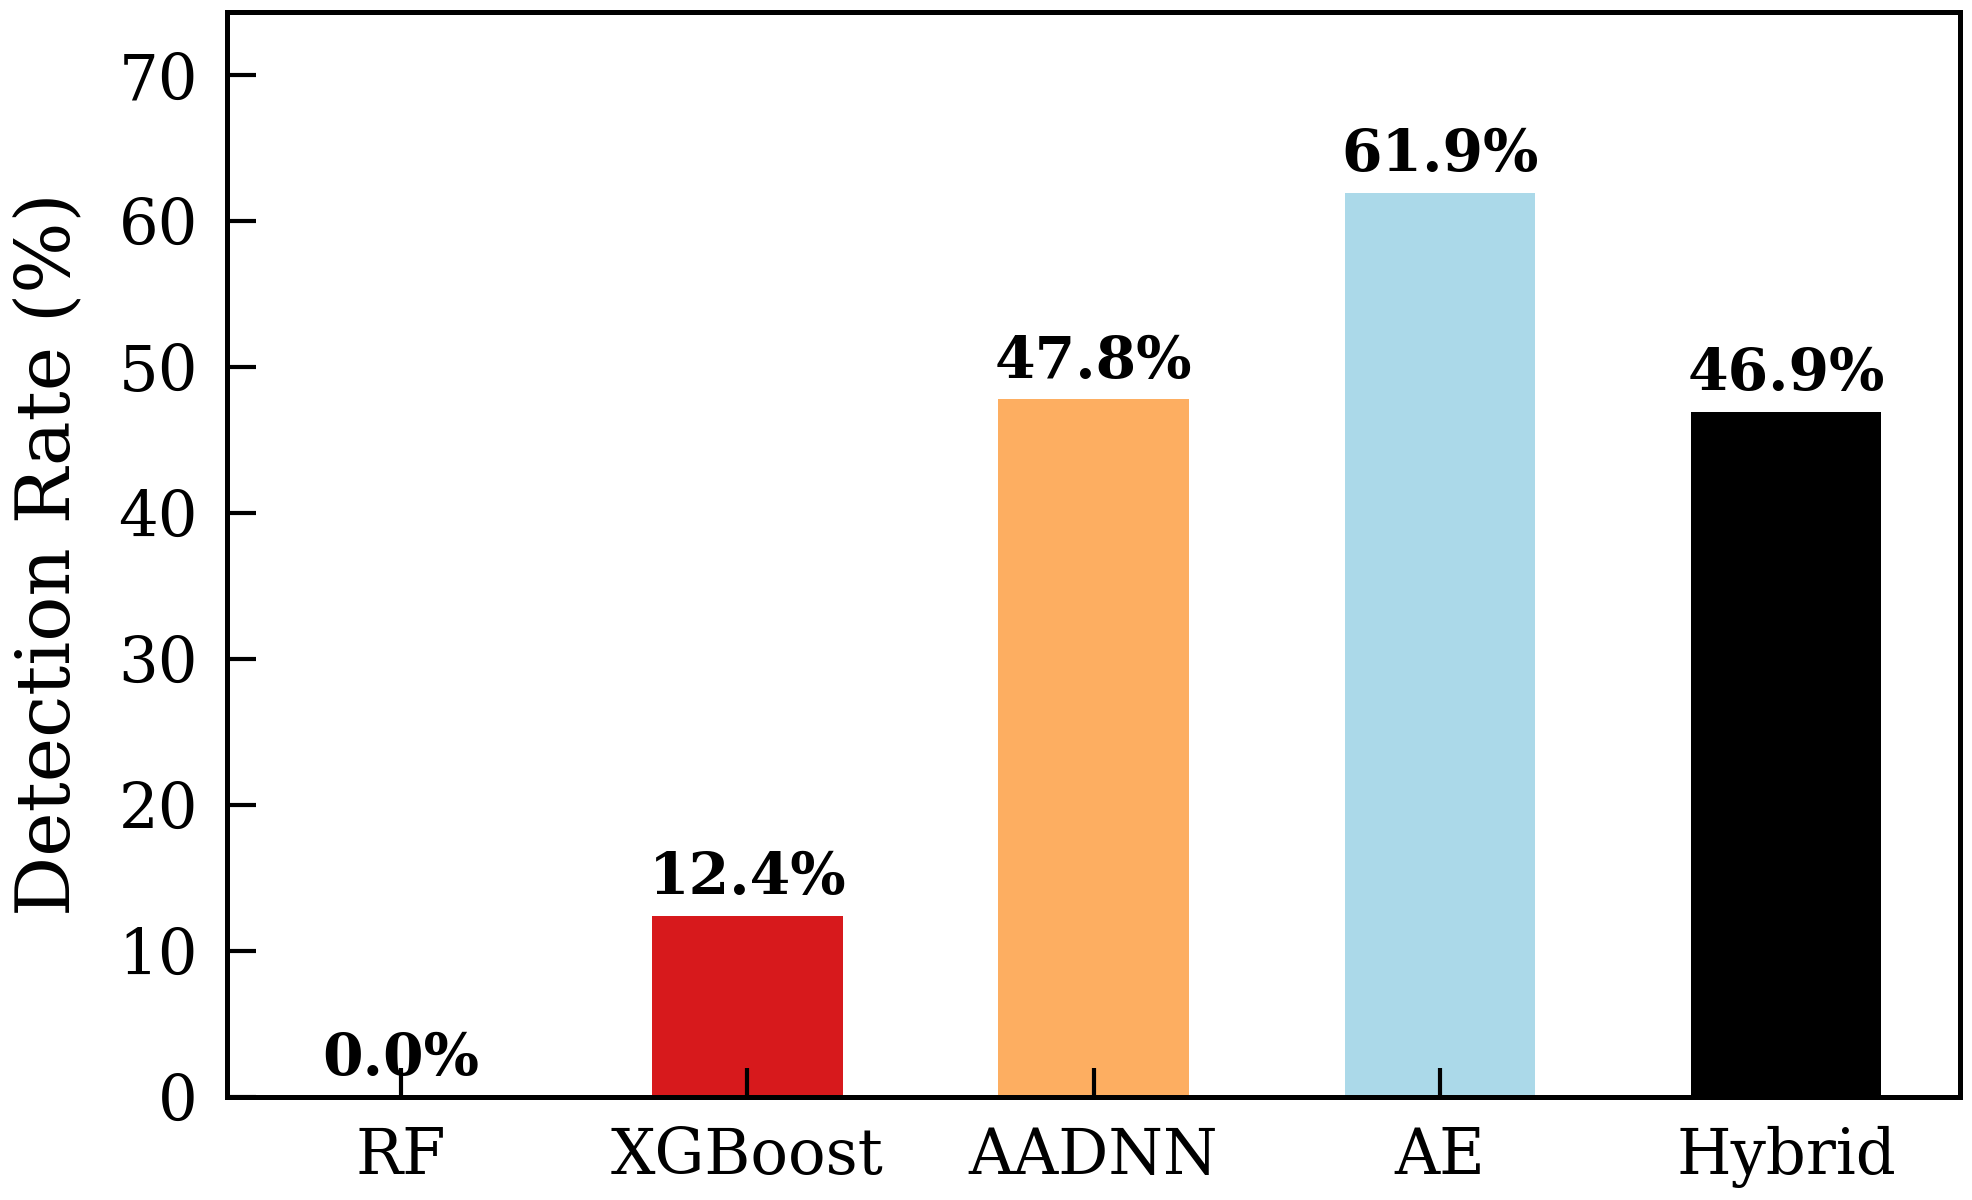
\includegraphics[width=0.88\columnwidth]{fig10_novel.png}
\caption{Detection rates on novel fraud types not seen during training. Random Forest and XGBoost achieve near zero detection, demonstrating the fundamental limitation of purely supervised approaches. The autoencoder branch enables the Hybrid model to detect 46.9\% of novel attacks.}
\label{fig:novel}
\end{figure}

RF detects 0.0\% and XGBoost only 12.4\% of novel fraud, confirming that supervised models are fundamentally unable to detect attacks absent from the training distribution. The Autoencoder achieves the highest novel detection (61.9\%) through reconstruction error, while the Hybrid reaches 46.9\%. This result demonstrates that even when supervised models achieve high AUC on known patterns, they provide no protection against emerging threats, whereas the unsupervised branch fills this critical gap.

\subsection{Overall Classification Performance}

Table~\ref{tab:main} presents performance metrics averaged over three seeds. The proposed Hybrid achieves the highest ROC AUC ($0.965 \pm 0.004$), exceeding RF ($0.959$), XGBoost ($0.937$), and both standalone components. Under dynamic thresholding, $F_1$ reaches 0.886, competitive with RF (0.895) and XGBoost (0.897). The ROC and PR curves from the primary run (seed 42) are shown in Figs.~\ref{fig:roc} and~\ref{fig:pr}.

\begin{table}[!t]
\centering
\caption{Performance Comparison (Mean $\pm$ Std, 3 Seeds)}
\label{tab:main}
\begin{tabular}{@{}lcccc@{}}
\toprule
\textbf{Model} & \textbf{AUC} & \textbf{PR AUC} & \textbf{$F_1$} & \textbf{Recall} \\
\midrule
RF       & $.959{\pm}.003$ & $\mathbf{.879{\pm}.009}$ & $.895{\pm}.014$ & $.833$ \\
XGBoost  & $.937{\pm}.007$ & $.859{\pm}.007$ & $.897{\pm}.013$ & $.841$ \\
AADNN    & $.930{\pm}.018$ & $.839{\pm}.018$ & $.871{\pm}.005$ & $.799$ \\
AE       & $.958{\pm}.003$ & $.507{\pm}.146$ & $.662{\pm}.099$ & $.748$ \\
\textbf{Hybrid} & $\mathbf{.965{\pm}.004}$ & $.846{\pm}.018$ & $.871{\pm}.007$ & $.804$ \\
Hybrid+Dyn & $.965{\pm}.004$ & $.846{\pm}.018$ & $.886$ & $.819$ \\
\bottomrule
\end{tabular}
\end{table}

\begin{figure}[!t]
\centering
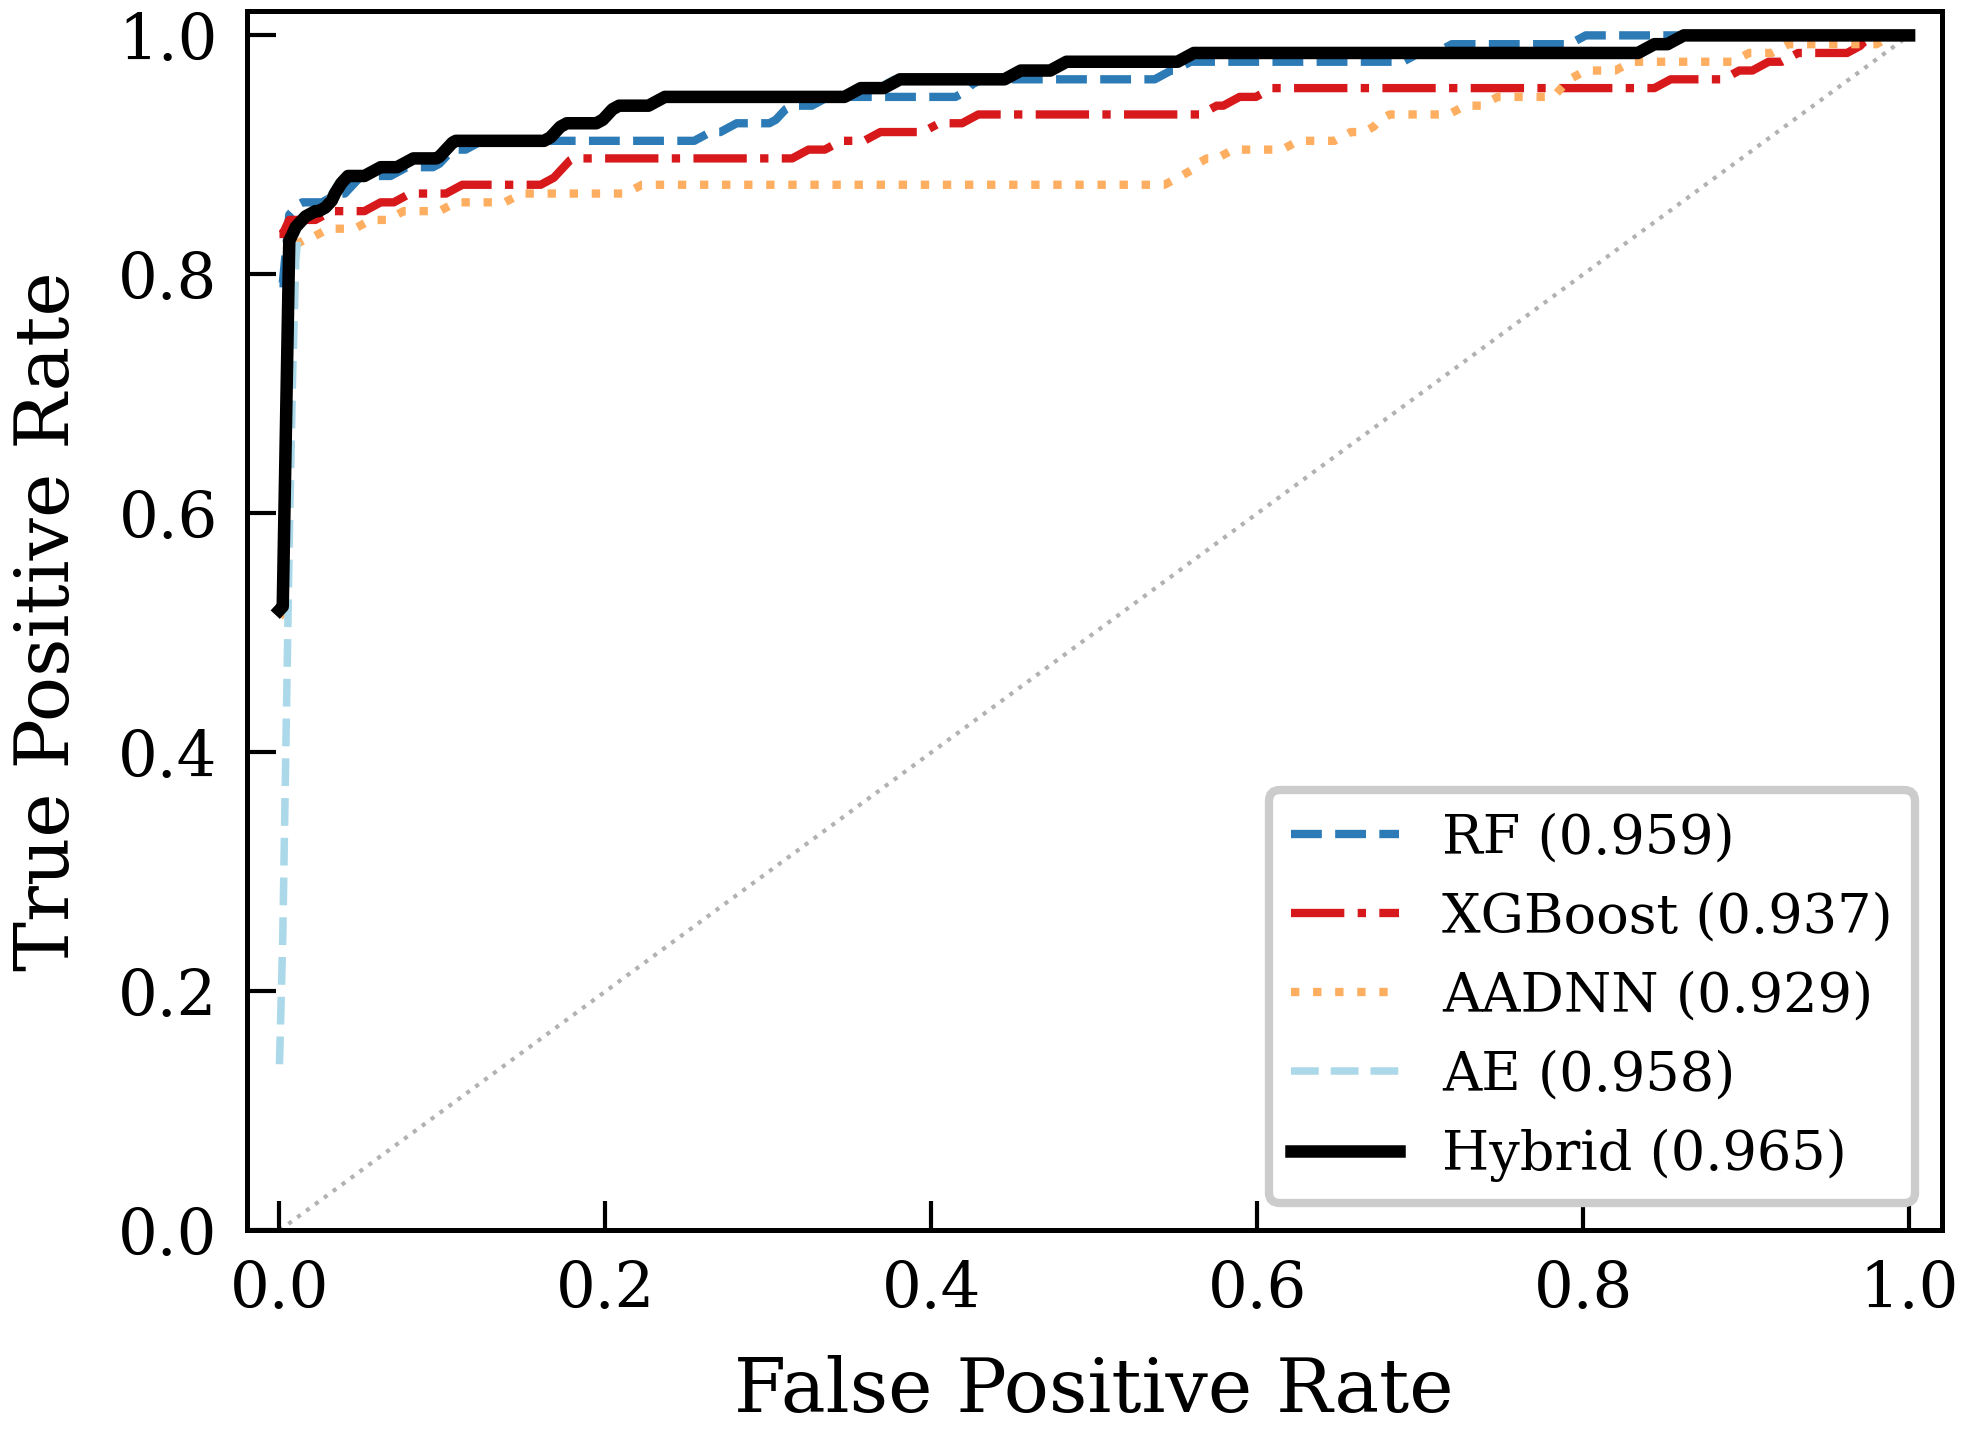
\includegraphics[width=\columnwidth]{fig01_roc.png}
\caption{ROC curves (seed 42). Legend values are cross seed means from Table~\ref{tab:main}. The Hybrid model (black, solid line) achieves the highest AUC among all methods.}
\label{fig:roc}
\end{figure}

\begin{figure}[!t]
\centering
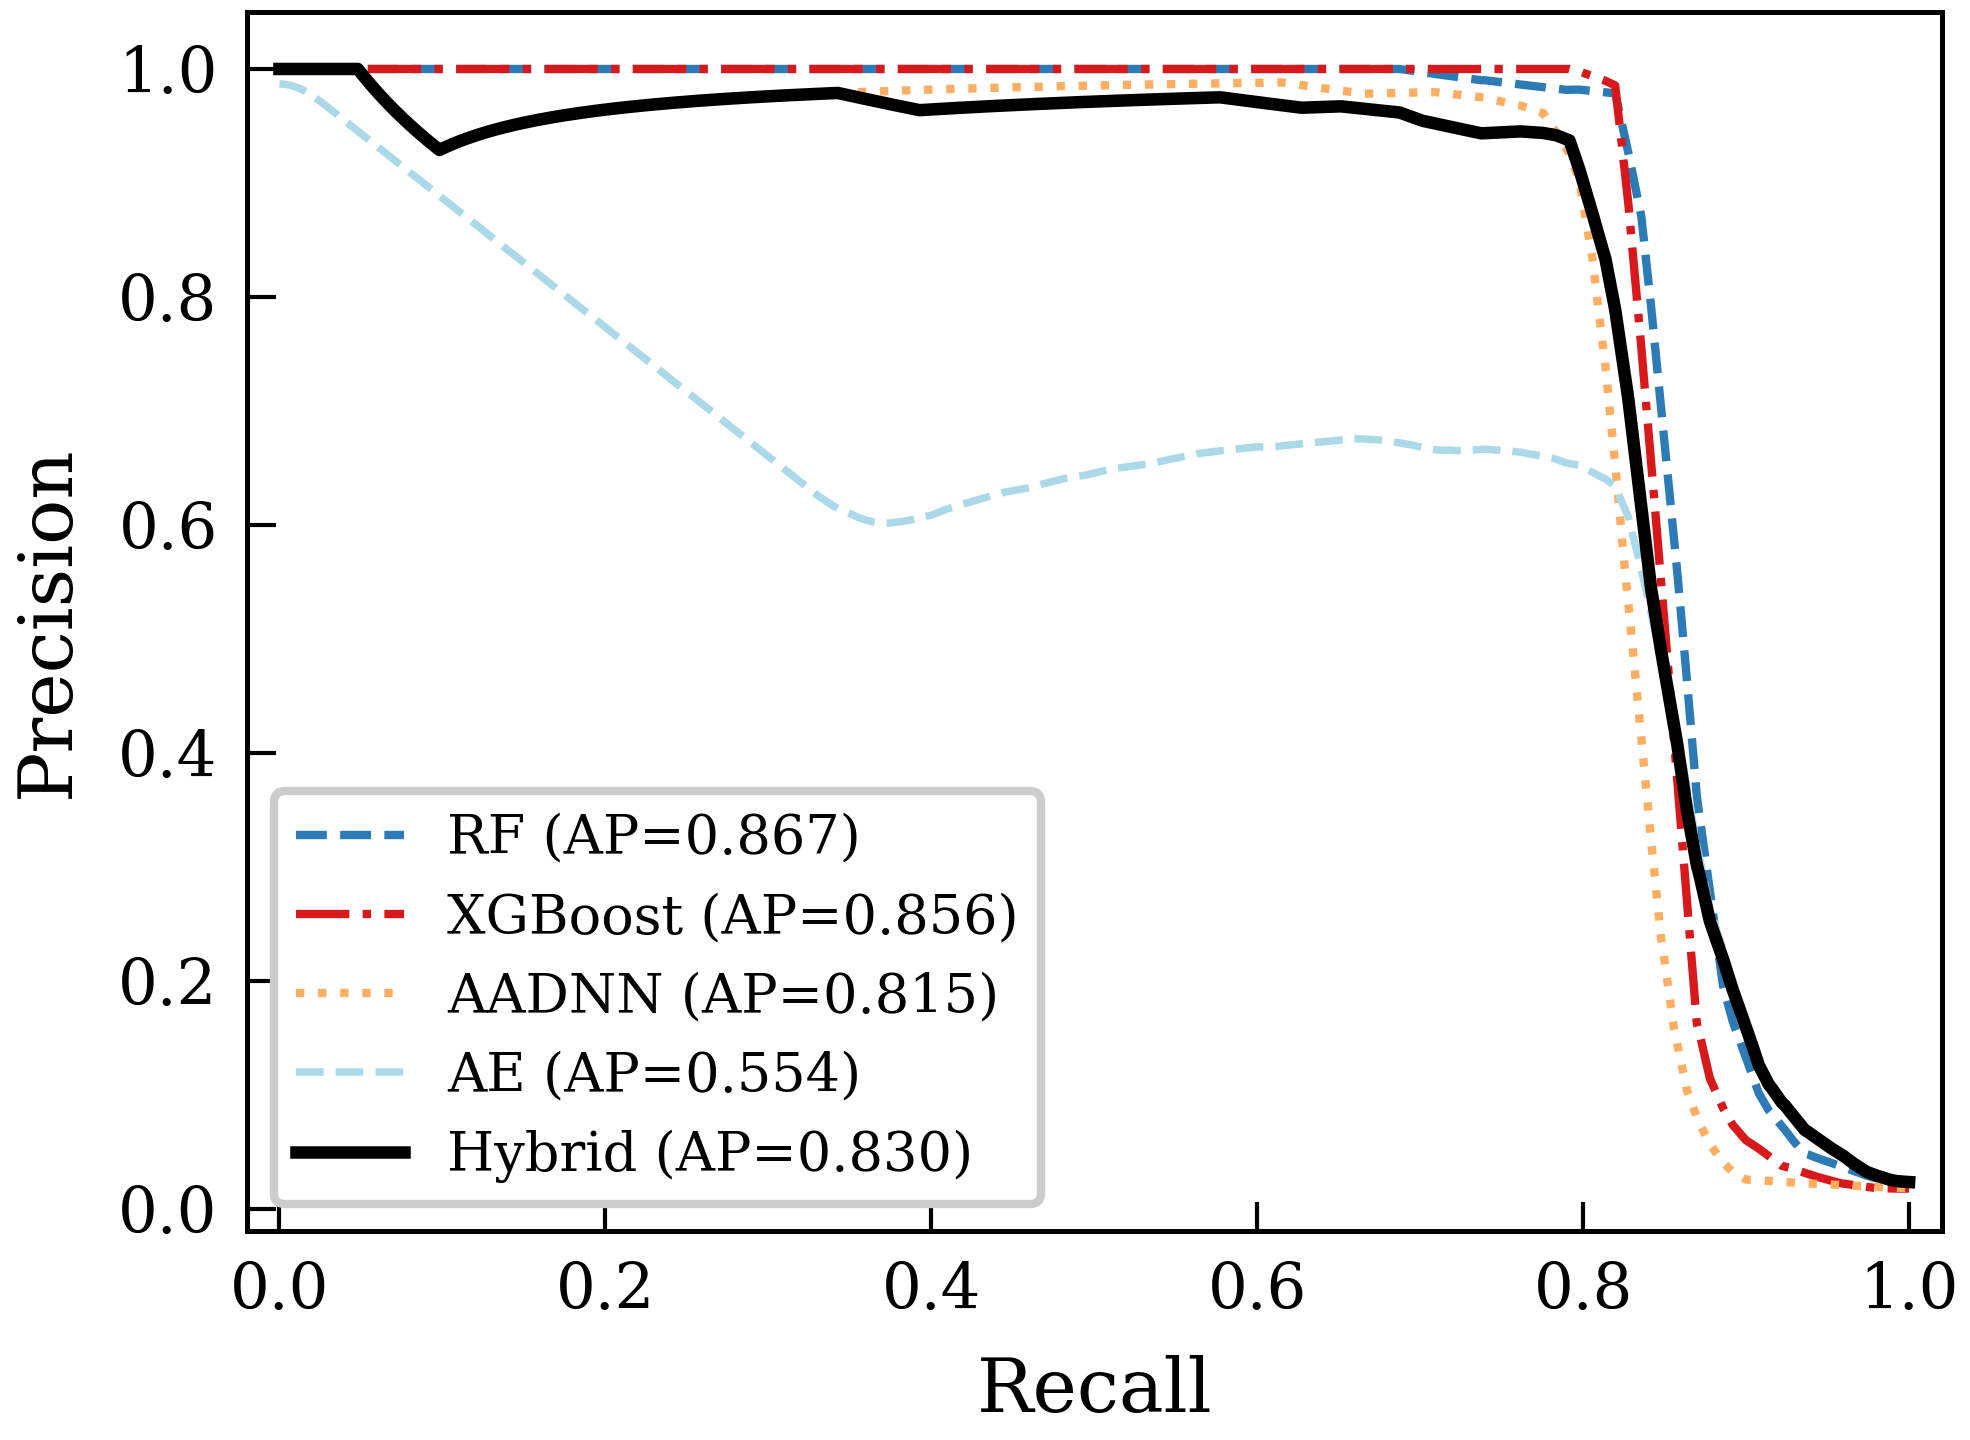
\includegraphics[width=\columnwidth]{fig02_pr.png}
\caption{Precision Recall curves with Average Precision. While RF achieves slightly higher AP on known fraud patterns, this advantage is offset by its inability to detect novel fraud (Table~\ref{tab:novel}).}
\label{fig:pr}
\end{figure}

The Hybrid's primary advantage is not marginal metric improvement on known fraud patterns, but rather the combination of competitive known fraud performance with novel fraud capability (Table~\ref{tab:novel}), adaptive thresholding, and explainability. These three capabilities are absent from all baseline methods.

\subsection{Ablation Study}

Table~\ref{tab:ablation} and Fig.~\ref{fig:ablation} present the systematic ablation. Adding the AE branch to the AADNN improves AUC from 0.930 to 0.965 (+3.8\%), confirming that the unsupervised anomaly signal provides complementary discriminative information. Dynamic thresholding further improves $F_1$ from 0.871 to 0.886 (+1.7\%) and recall from 0.804 to 0.819 (+1.9\%).

\begin{table}[!t]
\centering
\caption{Ablation Study (Mean $\pm$ Std, 3 Seeds)}
\label{tab:ablation}
\begin{tabular}{@{}lccc@{}}
\toprule
\textbf{Configuration} & \textbf{AUC} & \textbf{$F_1$} & \textbf{Recall} \\
\midrule
AADNN only            & $.930{\pm}.018$ & $.871{\pm}.005$ & $.799$ \\
AE only               & $.958{\pm}.003$ & $.662{\pm}.099$ & $.748$ \\
AADNN+AE (static $\tau$) & $.965{\pm}.004$ & $.871{\pm}.007$ & $.804$ \\
AADNN+AE (dynamic $\tau$) & $\mathbf{.965{\pm}.004}$ & $\mathbf{.886}$ & $\mathbf{.819}$ \\
\bottomrule
\end{tabular}
\end{table}

\begin{figure}[!t]
\centering
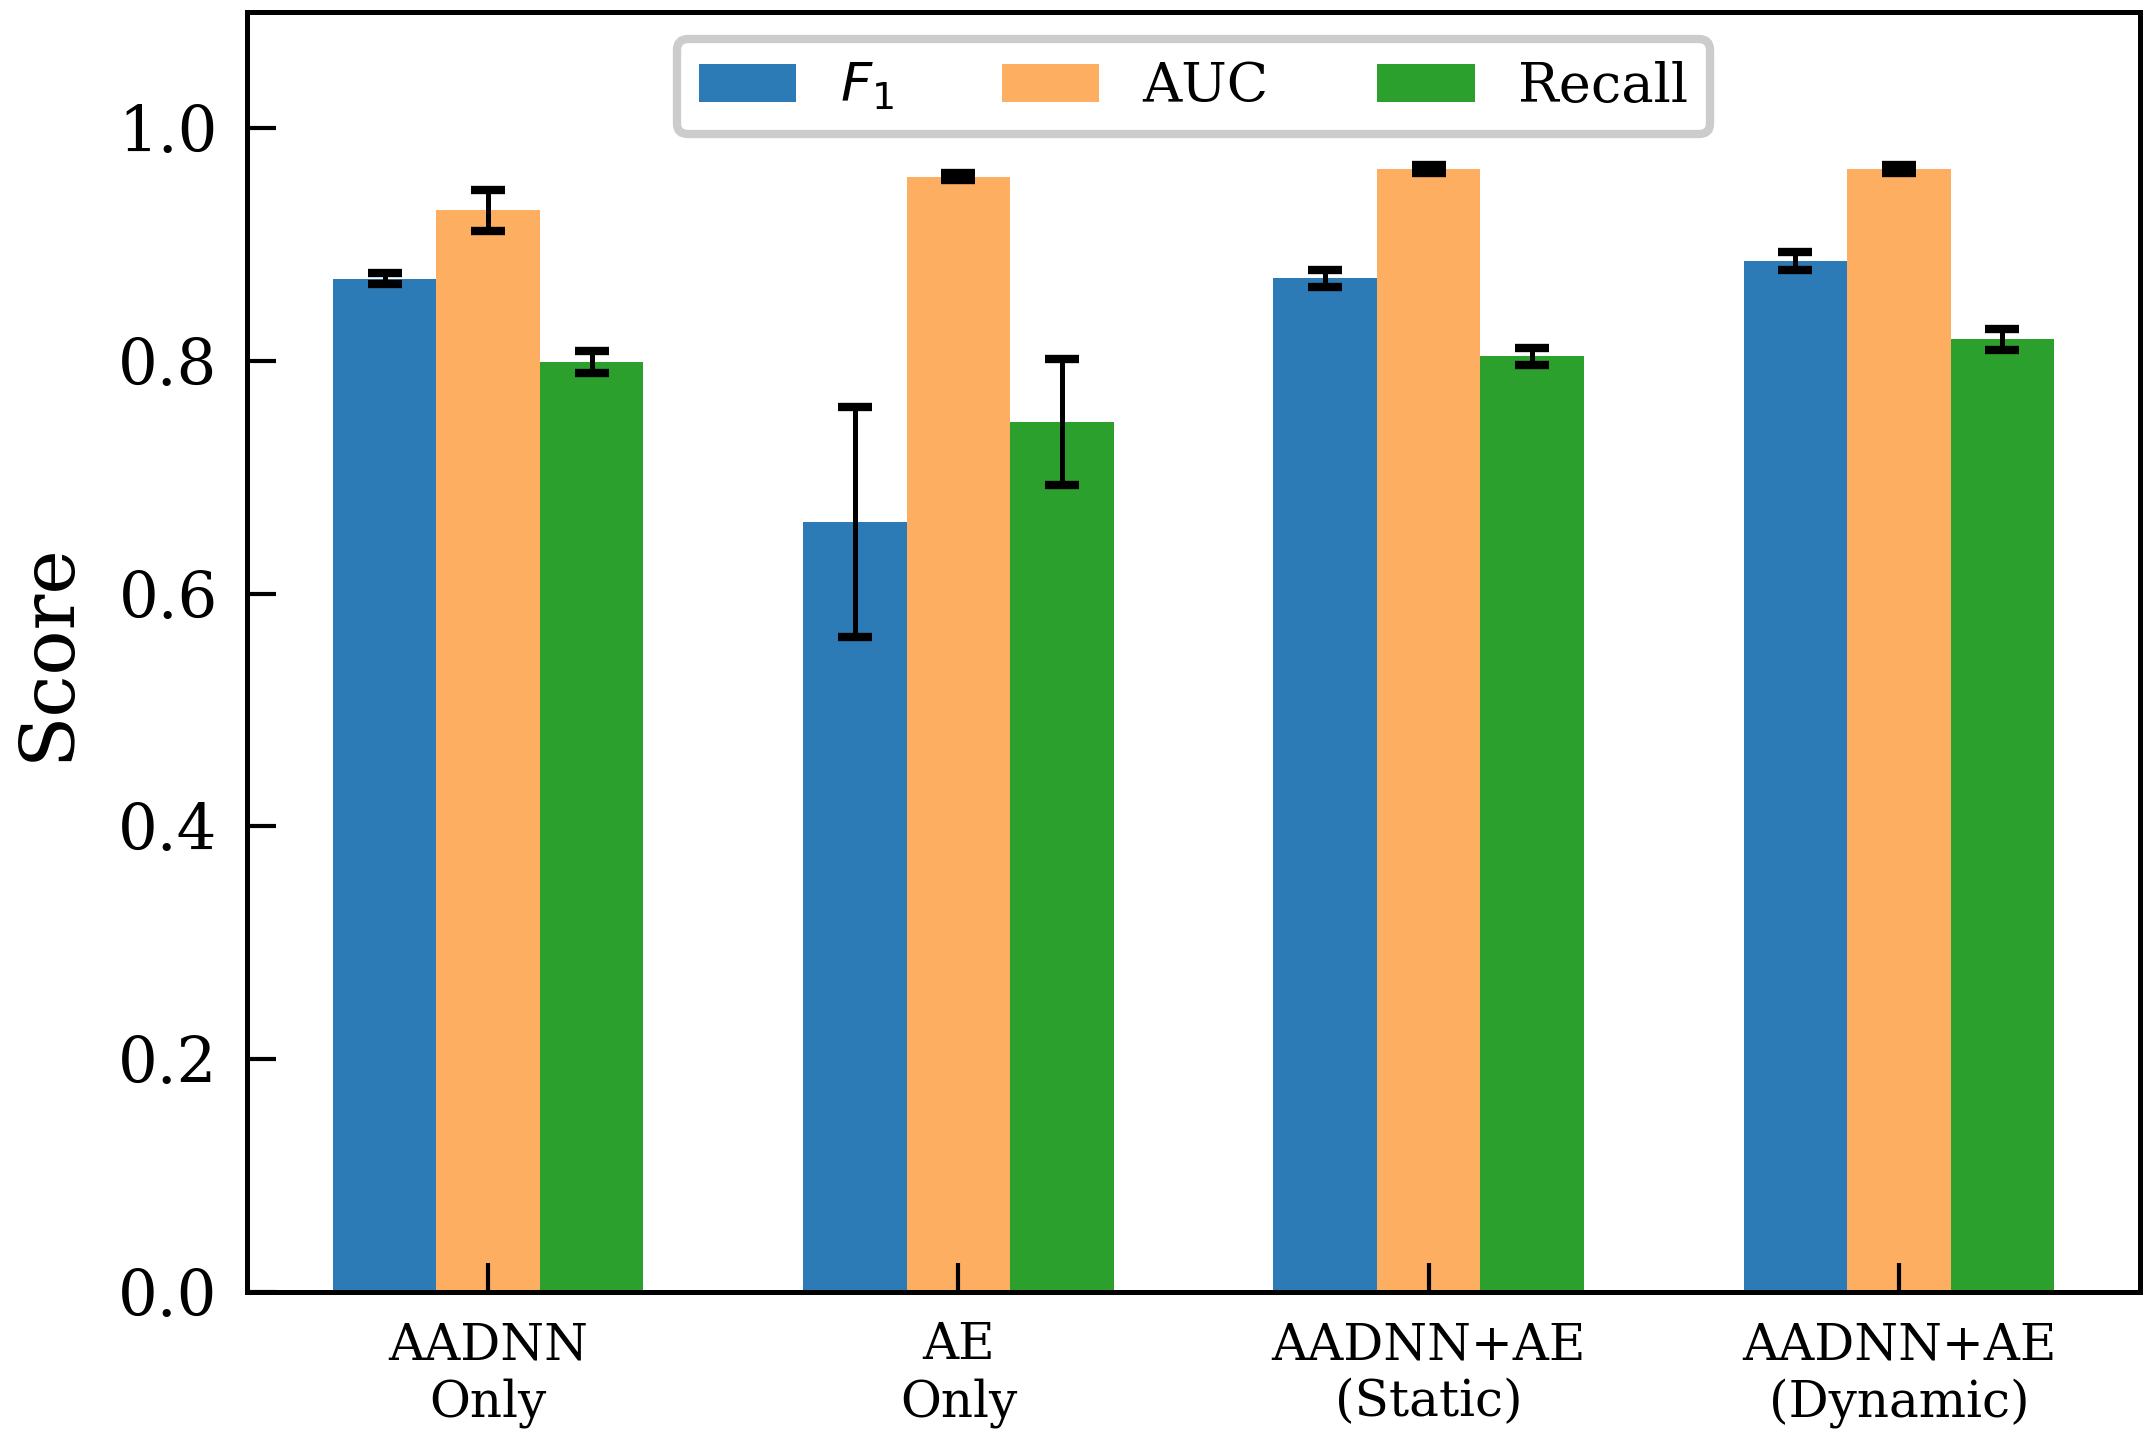
\includegraphics[width=\columnwidth]{fig09_ablation.png}
\caption{Ablation study with error bars across $F_1$, AUC, and Recall. Each added component provides measurable improvement, with dynamic thresholding contributing the largest recall gain (+1.9\%).}
\label{fig:ablation}
\end{figure}

\subsection{Hybrid Weight Optimization}

Fig.~\ref{fig:alpha} shows AUC as a function of the fusion weight $\alpha$. The optimal value $\alpha^* = 0.37$ indicates that the autoencoder contributes approximately 63\% of the fusion, reflecting the strong unsupervised separation in the PCA feature space. The broad plateau around the optimum (0.35--0.60) indicates robustness to moderate deviations in $\alpha$.

\begin{figure}[!t]
\centering
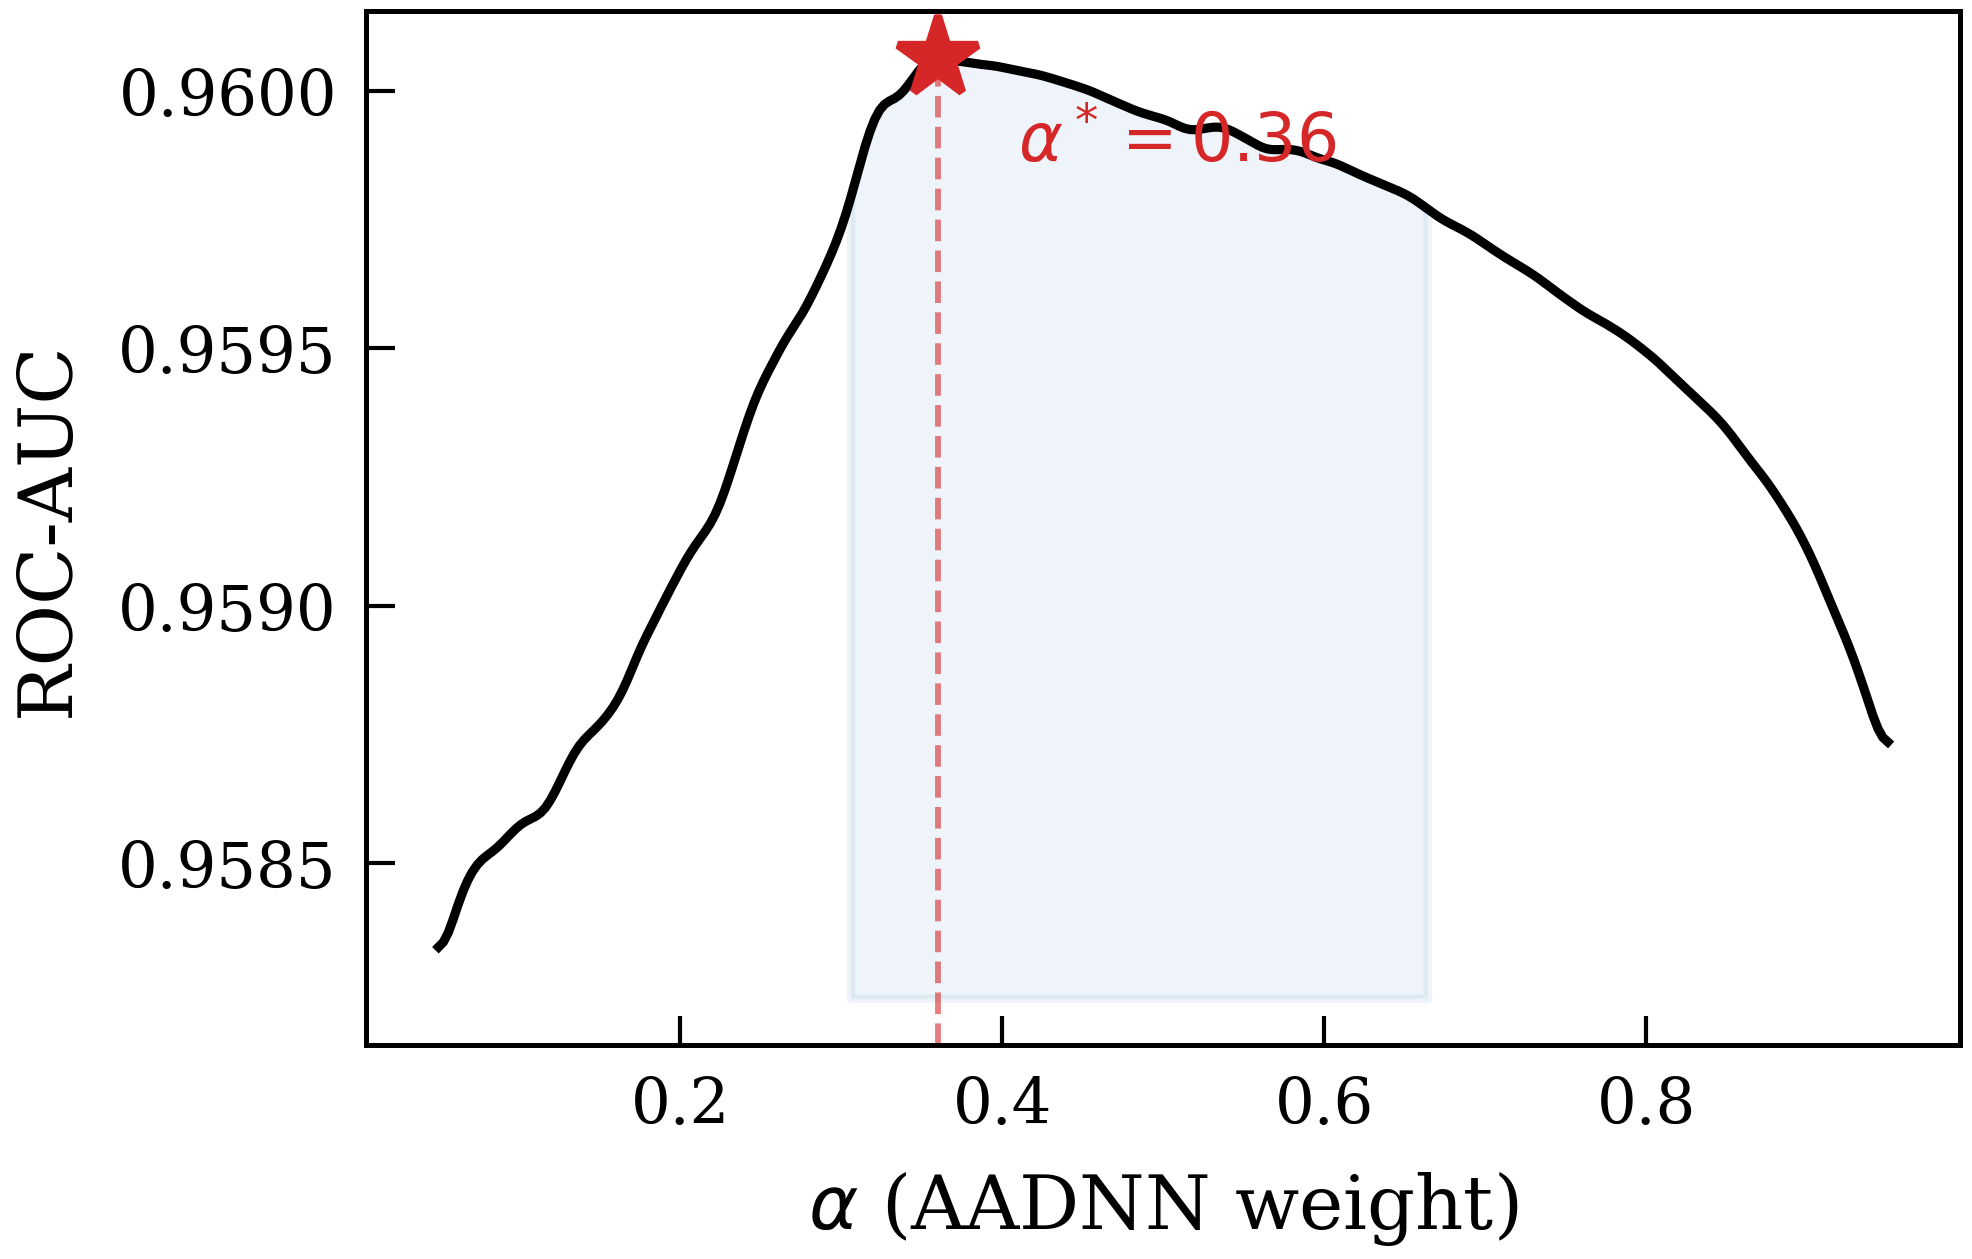
\includegraphics[width=0.88\columnwidth]{fig03_alpha.png}
\caption{ROC AUC as a function of fusion weight $\alpha$. Optimal $\alpha^*\!=\!0.37$. The broad plateau indicates robustness to the weight setting.}
\label{fig:alpha}
\end{figure}

\subsection{Dynamic Thresholding}

Table~\ref{tab:thresh} compares static and dynamic strategies. Dynamic thresholding improves $F_1$ from 0.871 to 0.886 (+1.7\%) and recall from 0.804 to 0.819 (+1.9\%). Fig.~\ref{fig:dyn} shows per window thresholds alongside fraud rates, confirming the expected inverse relationship: during high fraud periods, the threshold decreases to capture more positives, while during low fraud periods it increases to reduce false alarms.

\begin{table}[!t]
\centering
\caption{Static vs. Dynamic Threshold Performance}
\label{tab:thresh}
\begin{tabular}{@{}lccc@{}}
\toprule
\textbf{Strategy} & \textbf{Precision} & \textbf{Recall} & \textbf{$F_1$} \\
\midrule
Static ($\tau$ fixed) & $0.952$ & $0.804$ & $0.871$ \\
\textbf{Dynamic ($\tau_t$ per window)} & $\mathbf{0.968}$ & $\mathbf{0.819}$ & $\mathbf{0.886}$ \\
\bottomrule
\end{tabular}
\end{table}

\begin{figure}[!t]
\centering
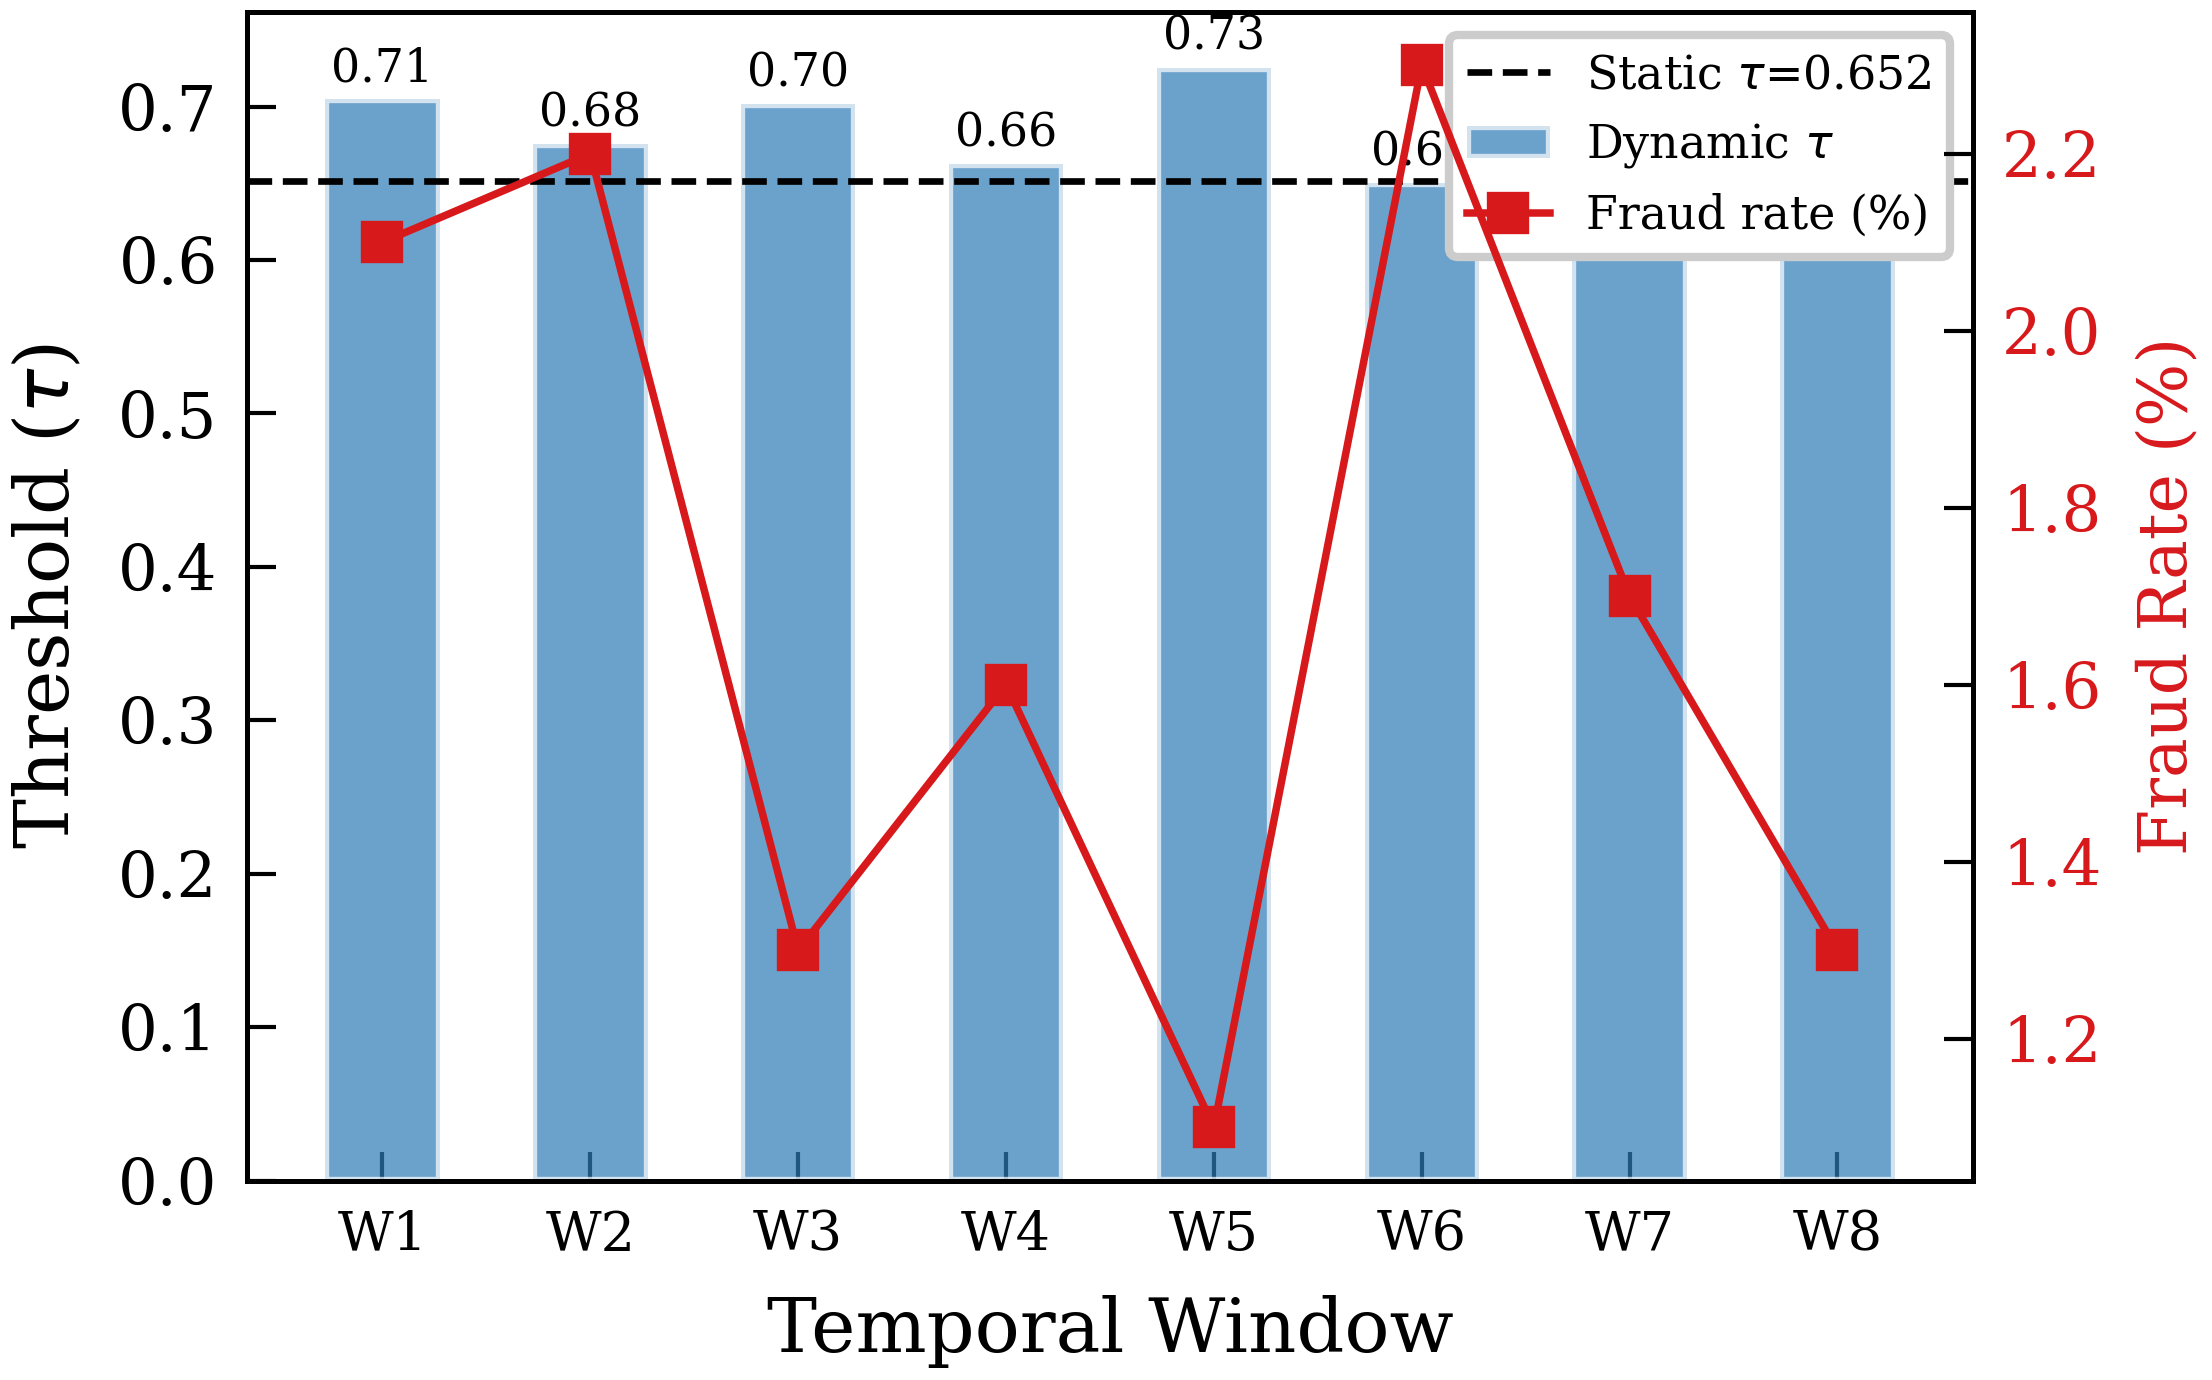
\includegraphics[width=\columnwidth]{fig05_dynamic.png}
\caption{Per window thresholds (bars) and fraud rates (line, right axis). Higher fraud periods require lower thresholds, and vice versa.}
\label{fig:dyn}
\end{figure}

\subsection{Autoencoder Error Analysis}

Fig.~\ref{fig:ae_dist} shows the distribution of autoencoder reconstruction errors with kernel density estimation overlays. Legitimate transactions cluster tightly around low error values, while fraudulent transactions produce significantly higher and more dispersed errors. The overlap region between the two distributions represents stealthy fraud cases that the supervised AADNN branch helps classify correctly.

\begin{figure}[!t]
\centering
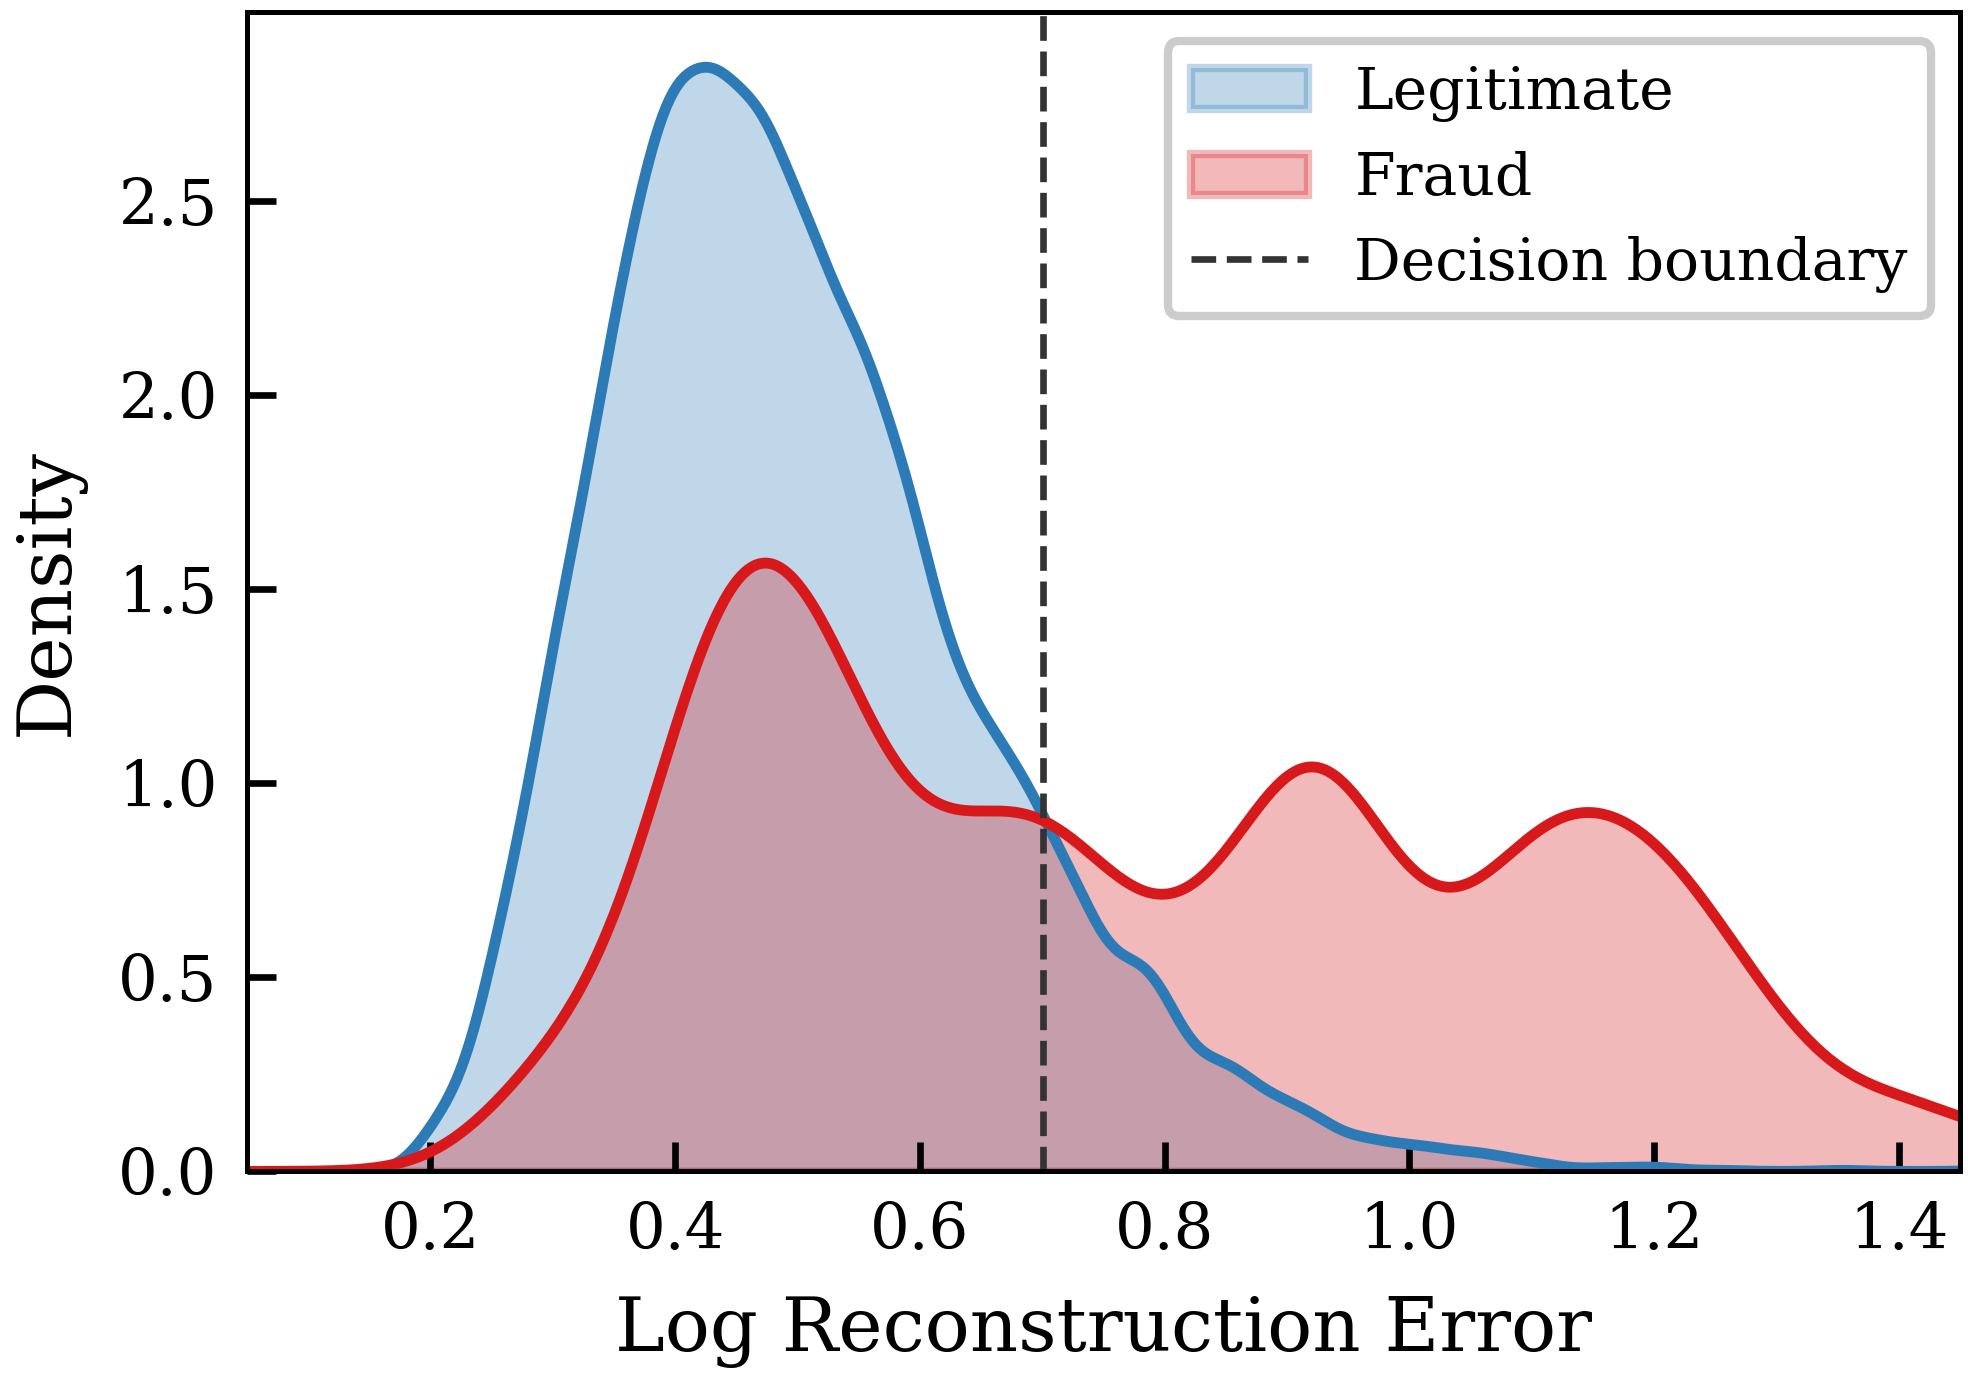
\includegraphics[width=0.88\columnwidth]{fig04_ae_dist.png}
\caption{Autoencoder reconstruction error distributions with KDE overlays. Fraud transactions produce higher, more dispersed errors, validating the anomaly detection principle.}
\label{fig:ae_dist}
\end{figure}

\subsection{Robustness Analysis}

Fig.~\ref{fig:robust} shows model performance under Gaussian noise injection at levels 0\% through 20\%, with confidence bands derived from the cross seed standard deviation. The Hybrid model degrades most gracefully (AUC drops from 0.960 to 0.958 at 20\% noise), while RF drops from 0.981 to 0.966. This stability stems from the dual branch architecture: even when noise degrades the AADNN, the autoencoder's reconstruction error based scoring remains robust to additive perturbations.

\begin{figure}[!t]
\centering
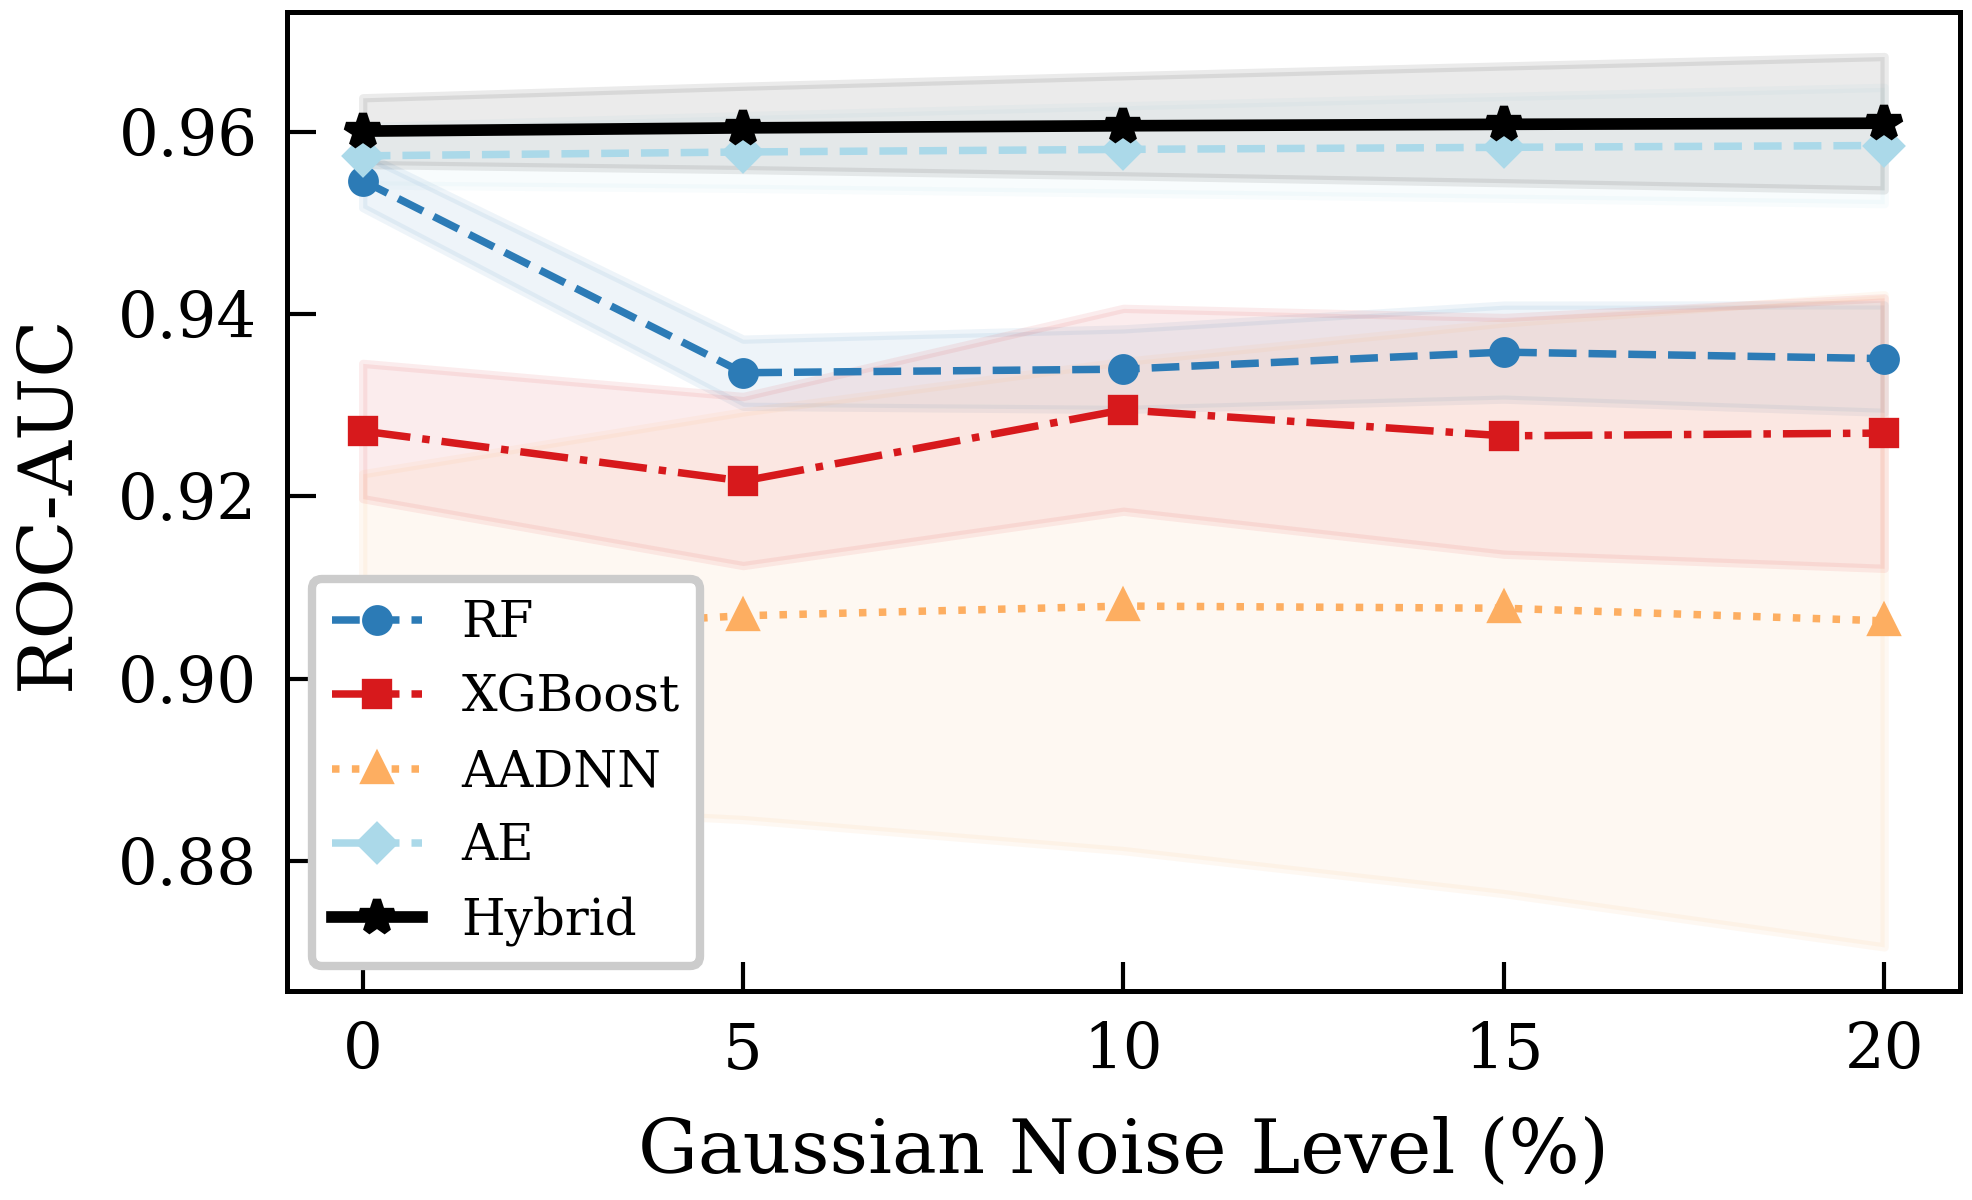
\includegraphics[width=0.88\columnwidth]{fig11_robust.png}
\caption{AUC under increasing Gaussian noise with confidence bands. The Hybrid model exhibits the smallest performance degradation across all noise levels.}
\label{fig:robust}
\end{figure}

\subsection{Cost Sensitivity Analysis}

Fig.~\ref{fig:cost} shows total financial cost under varying false negative multipliers $\lambda_{\text{FN}} \in \{0.25, 0.5, 1.0, 2.0\}$. The Hybrid achieves comparable financial cost to RF and XGBoost across all settings while additionally providing anomaly detection and explainability capabilities that pure ensemble methods lack. As $\lambda_{\text{FN}}$ increases (reflecting scenarios where missed fraud is more costly), the cost differences between models become more pronounced.

\begin{figure}[!t]
\centering
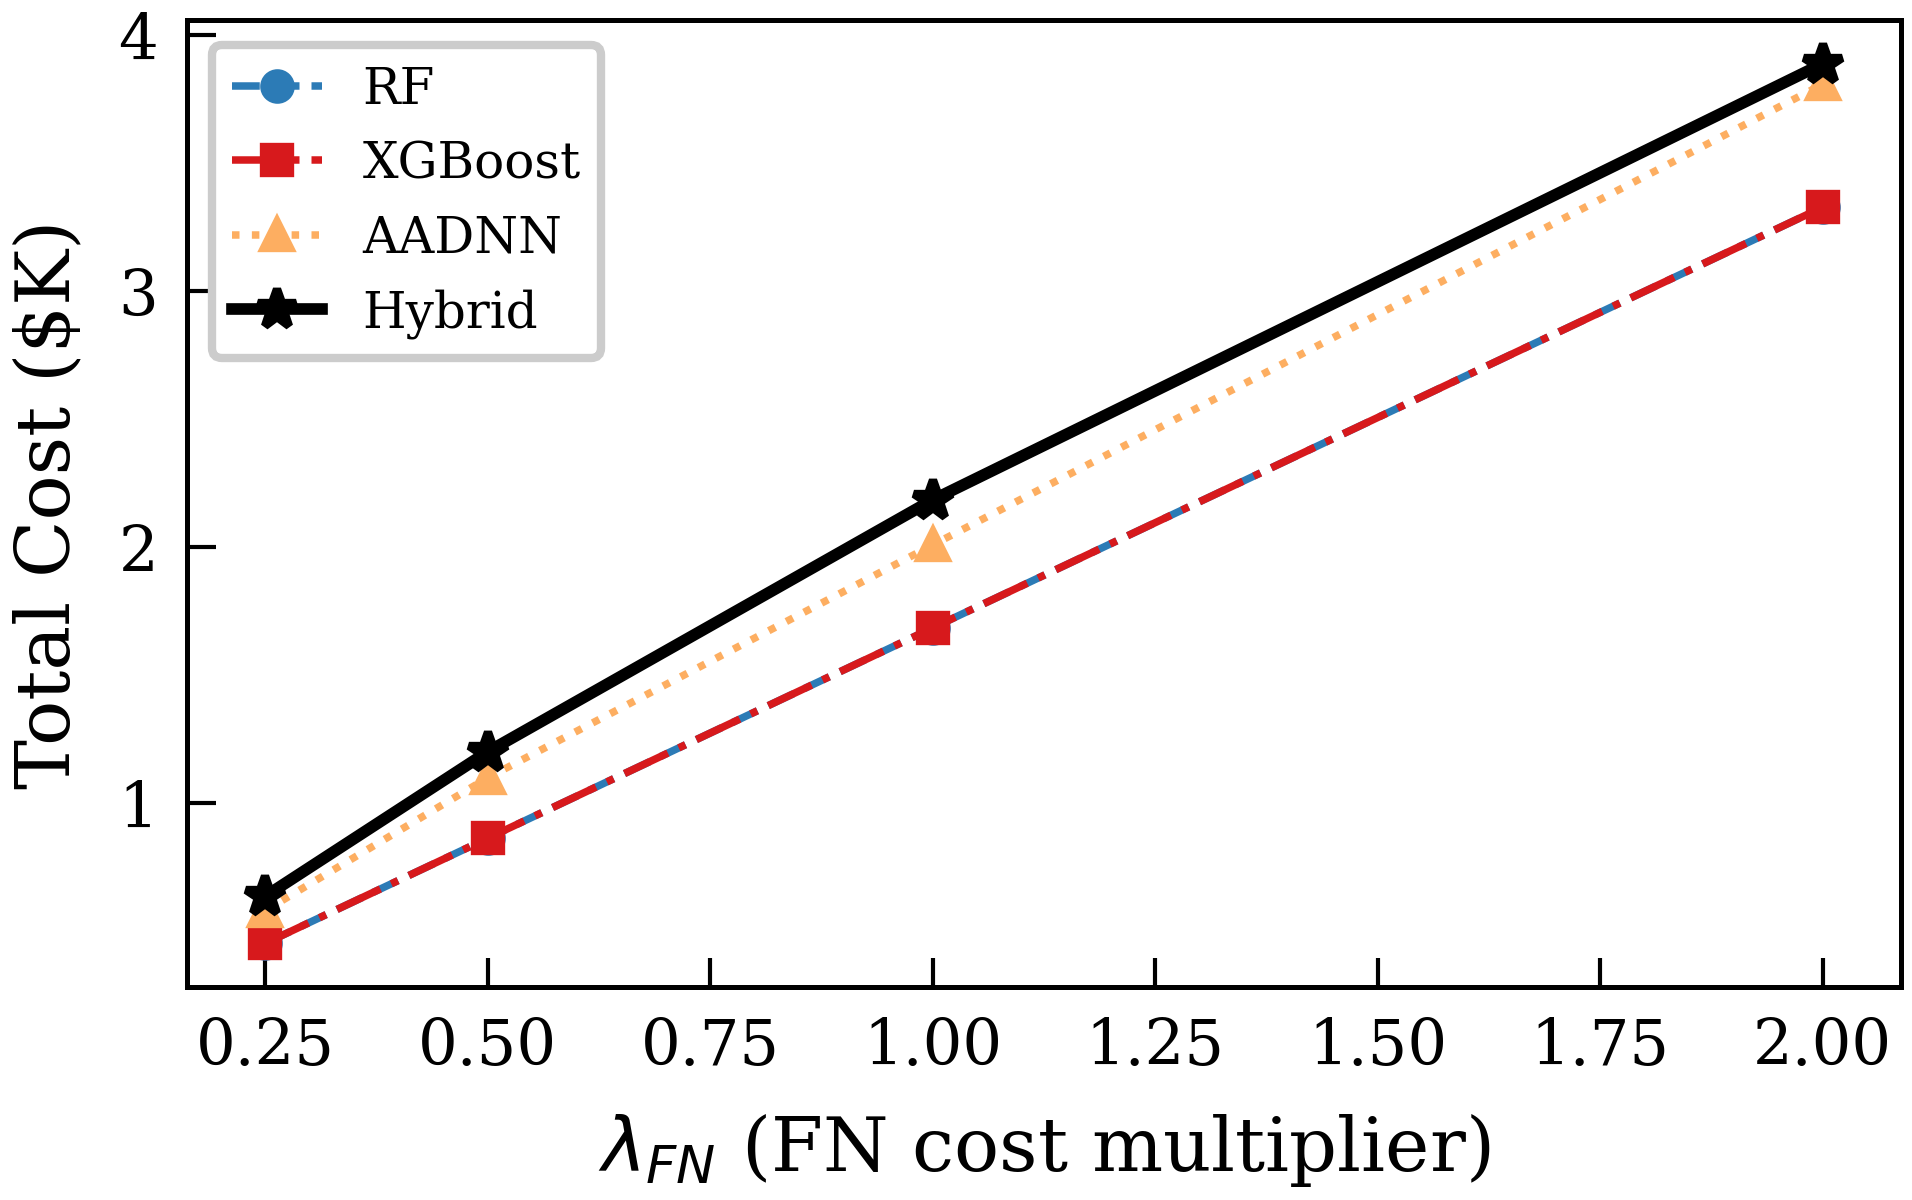
\includegraphics[width=0.88\columnwidth]{fig12_cost.png}
\caption{Total financial cost under varying false negative cost multipliers. All models scale approximately linearly; the Hybrid remains competitive.}
\label{fig:cost}
\end{figure}

\subsection{Computational Complexity}

Table~\ref{tab:timing} reports training times, inference latency, and approximate parameter counts. The Hybrid requires the longest training time (27.3s total) as it trains both the AADNN and autoencoder sequentially. However, inference time of 55.7ms for the entire test set of 8{,}000 transactions translates to less than 0.01ms per transaction, which is well within the latency budget for real time deployment at point of sale terminals.

\begin{table}[!t]
\centering
\caption{Computational Complexity}
\label{tab:timing}
\begin{tabular}{@{}lccc@{}}
\toprule
\textbf{Model} & \textbf{Train (s)} & \textbf{Inference (ms)} & \textbf{Parameters} \\
\midrule
RF       & 21.5  & 59.7 & 100 trees \\
XGBoost  & 2.0  & 17.0 & 150 estimators \\
AADNN    & 23.3 & 46.3 & ${\sim}$53K weights \\
AE       & 4.0 & 9.4 & ${\sim}$6K weights \\
Hybrid   & 27.3 & 55.7 & ${\sim}$59K weights \\
\bottomrule
\end{tabular}
\end{table}

\subsection{SHAP Explainability}

Fig.~\ref{fig:shap} ranks the top 10 features by mean absolute SHAP value. Feature energy ($V_{\text{magnitude}}$), which measures the coordinated deviation across all 28 PCA dimensions, is the strongest fraud indicator (SHAP = 3.30), followed by $V_3$ (1.39). This is consistent with domain knowledge: fraudulent transactions often exhibit anomalous patterns across multiple dimensions simultaneously, rather than deviating on any single feature. Temporal features (night transactions, hour) and transaction amount also rank highly.

\begin{figure}[!t]
\centering
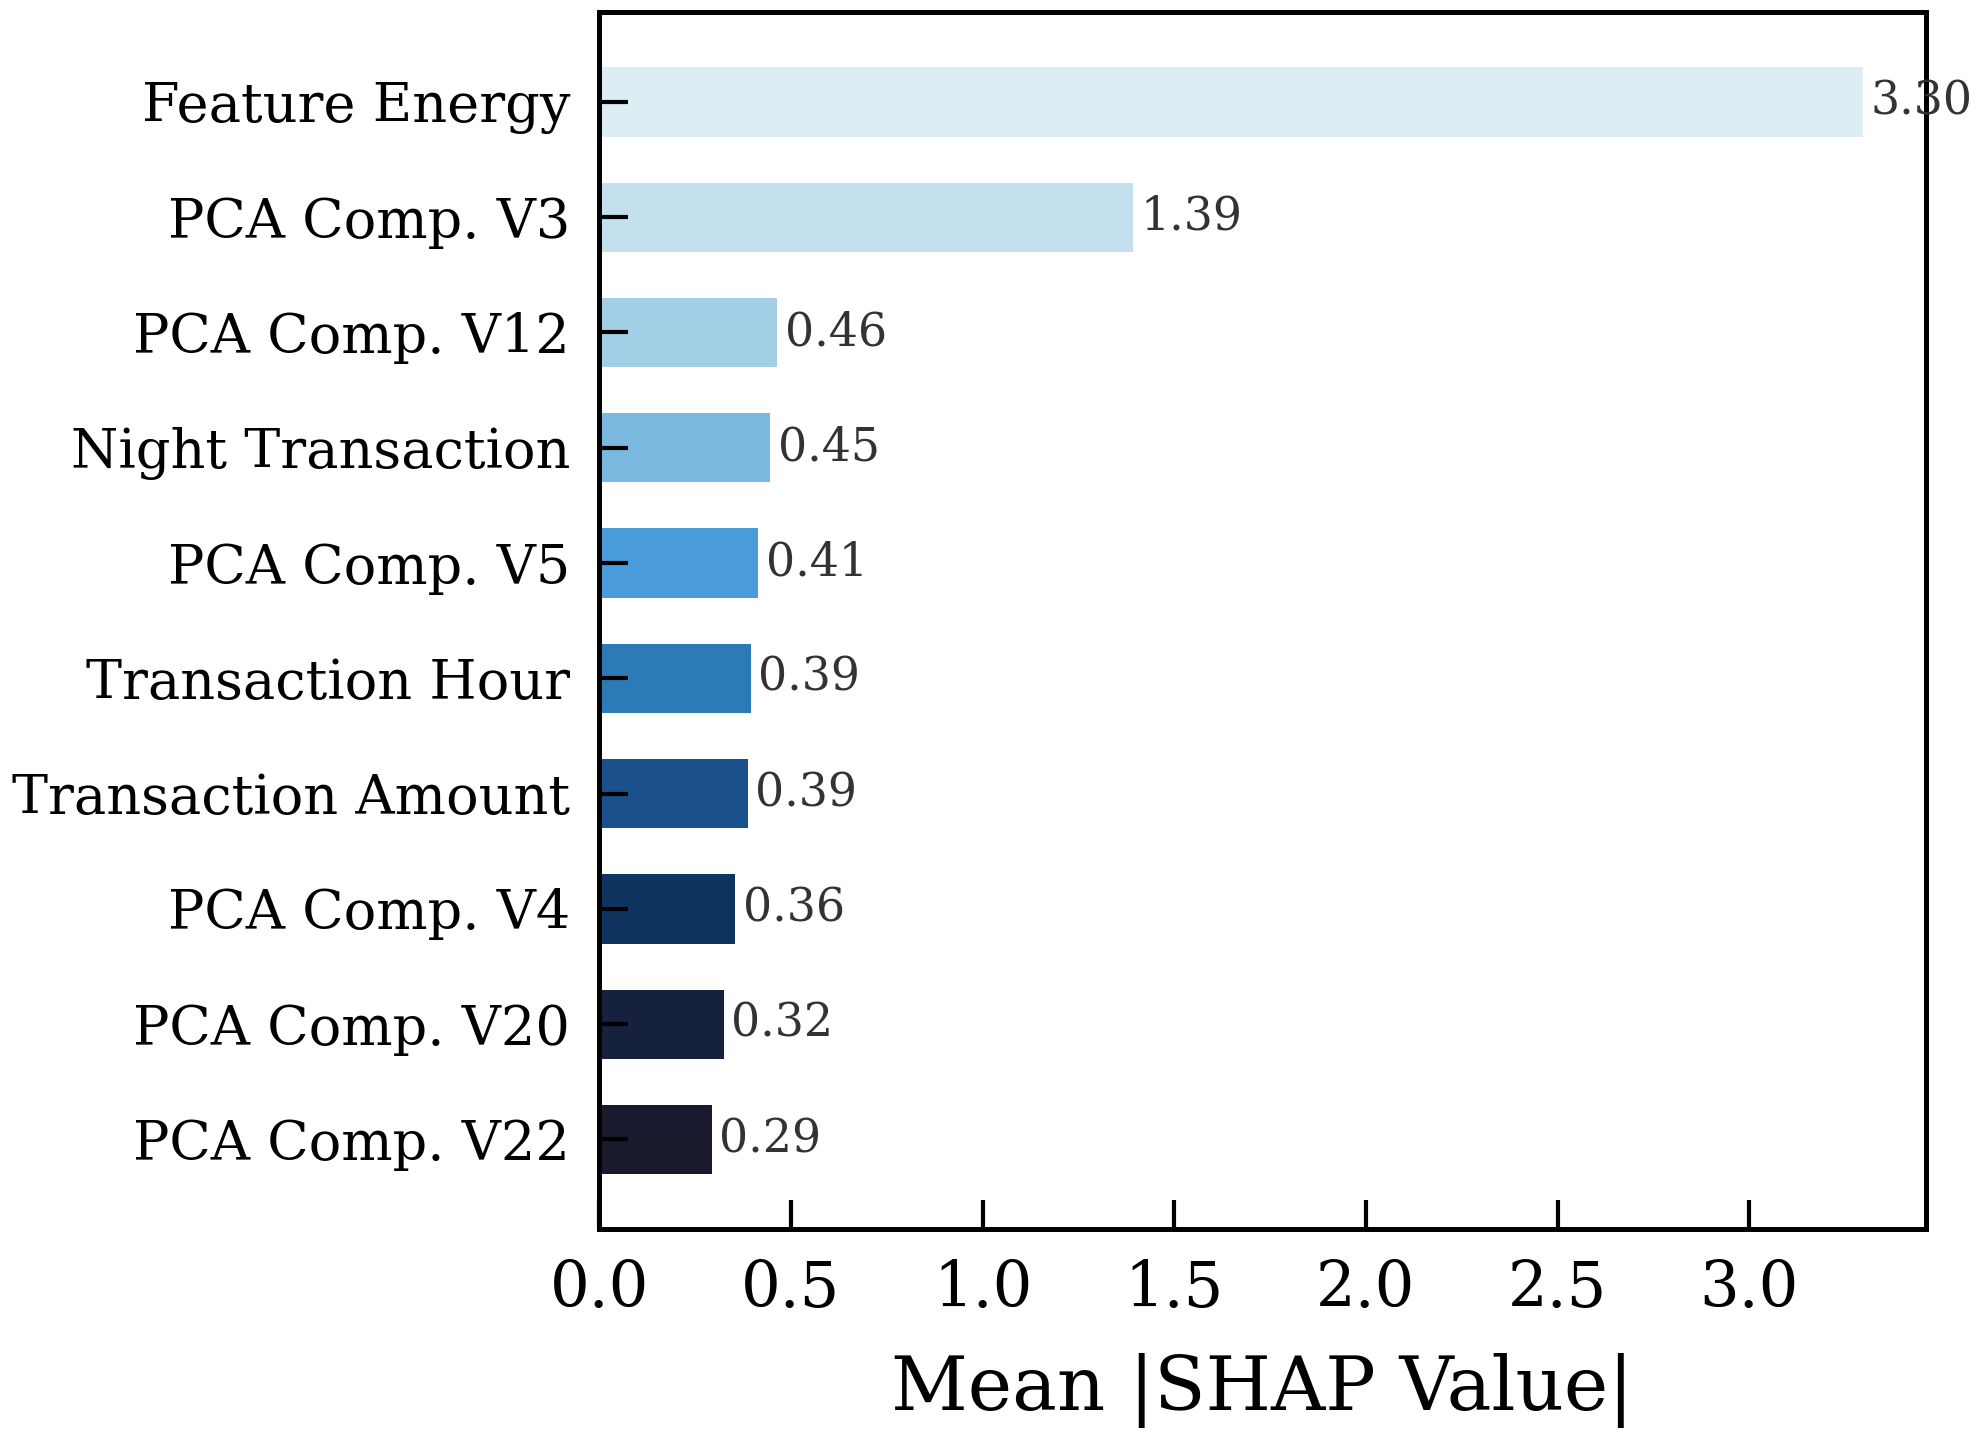
\includegraphics[width=0.88\columnwidth]{fig07_shap.png}
\caption{Top 10 features ranked by mean absolute SHAP value. Feature energy (coordinated PCA deviation) dominates, consistent with the multi dimensional nature of fraud signals.}
\label{fig:shap}
\end{figure}

Fig.~\ref{fig:shap_summary} presents the SHAP summary plot showing the directional impact of each feature. High feature energy and low $V_3$ push predictions toward fraud, while low energy and high $V_3$ push toward legitimate. Table~\ref{tab:shap} provides per transaction explanations for four representative cases.

\begin{figure}[!t]
\centering
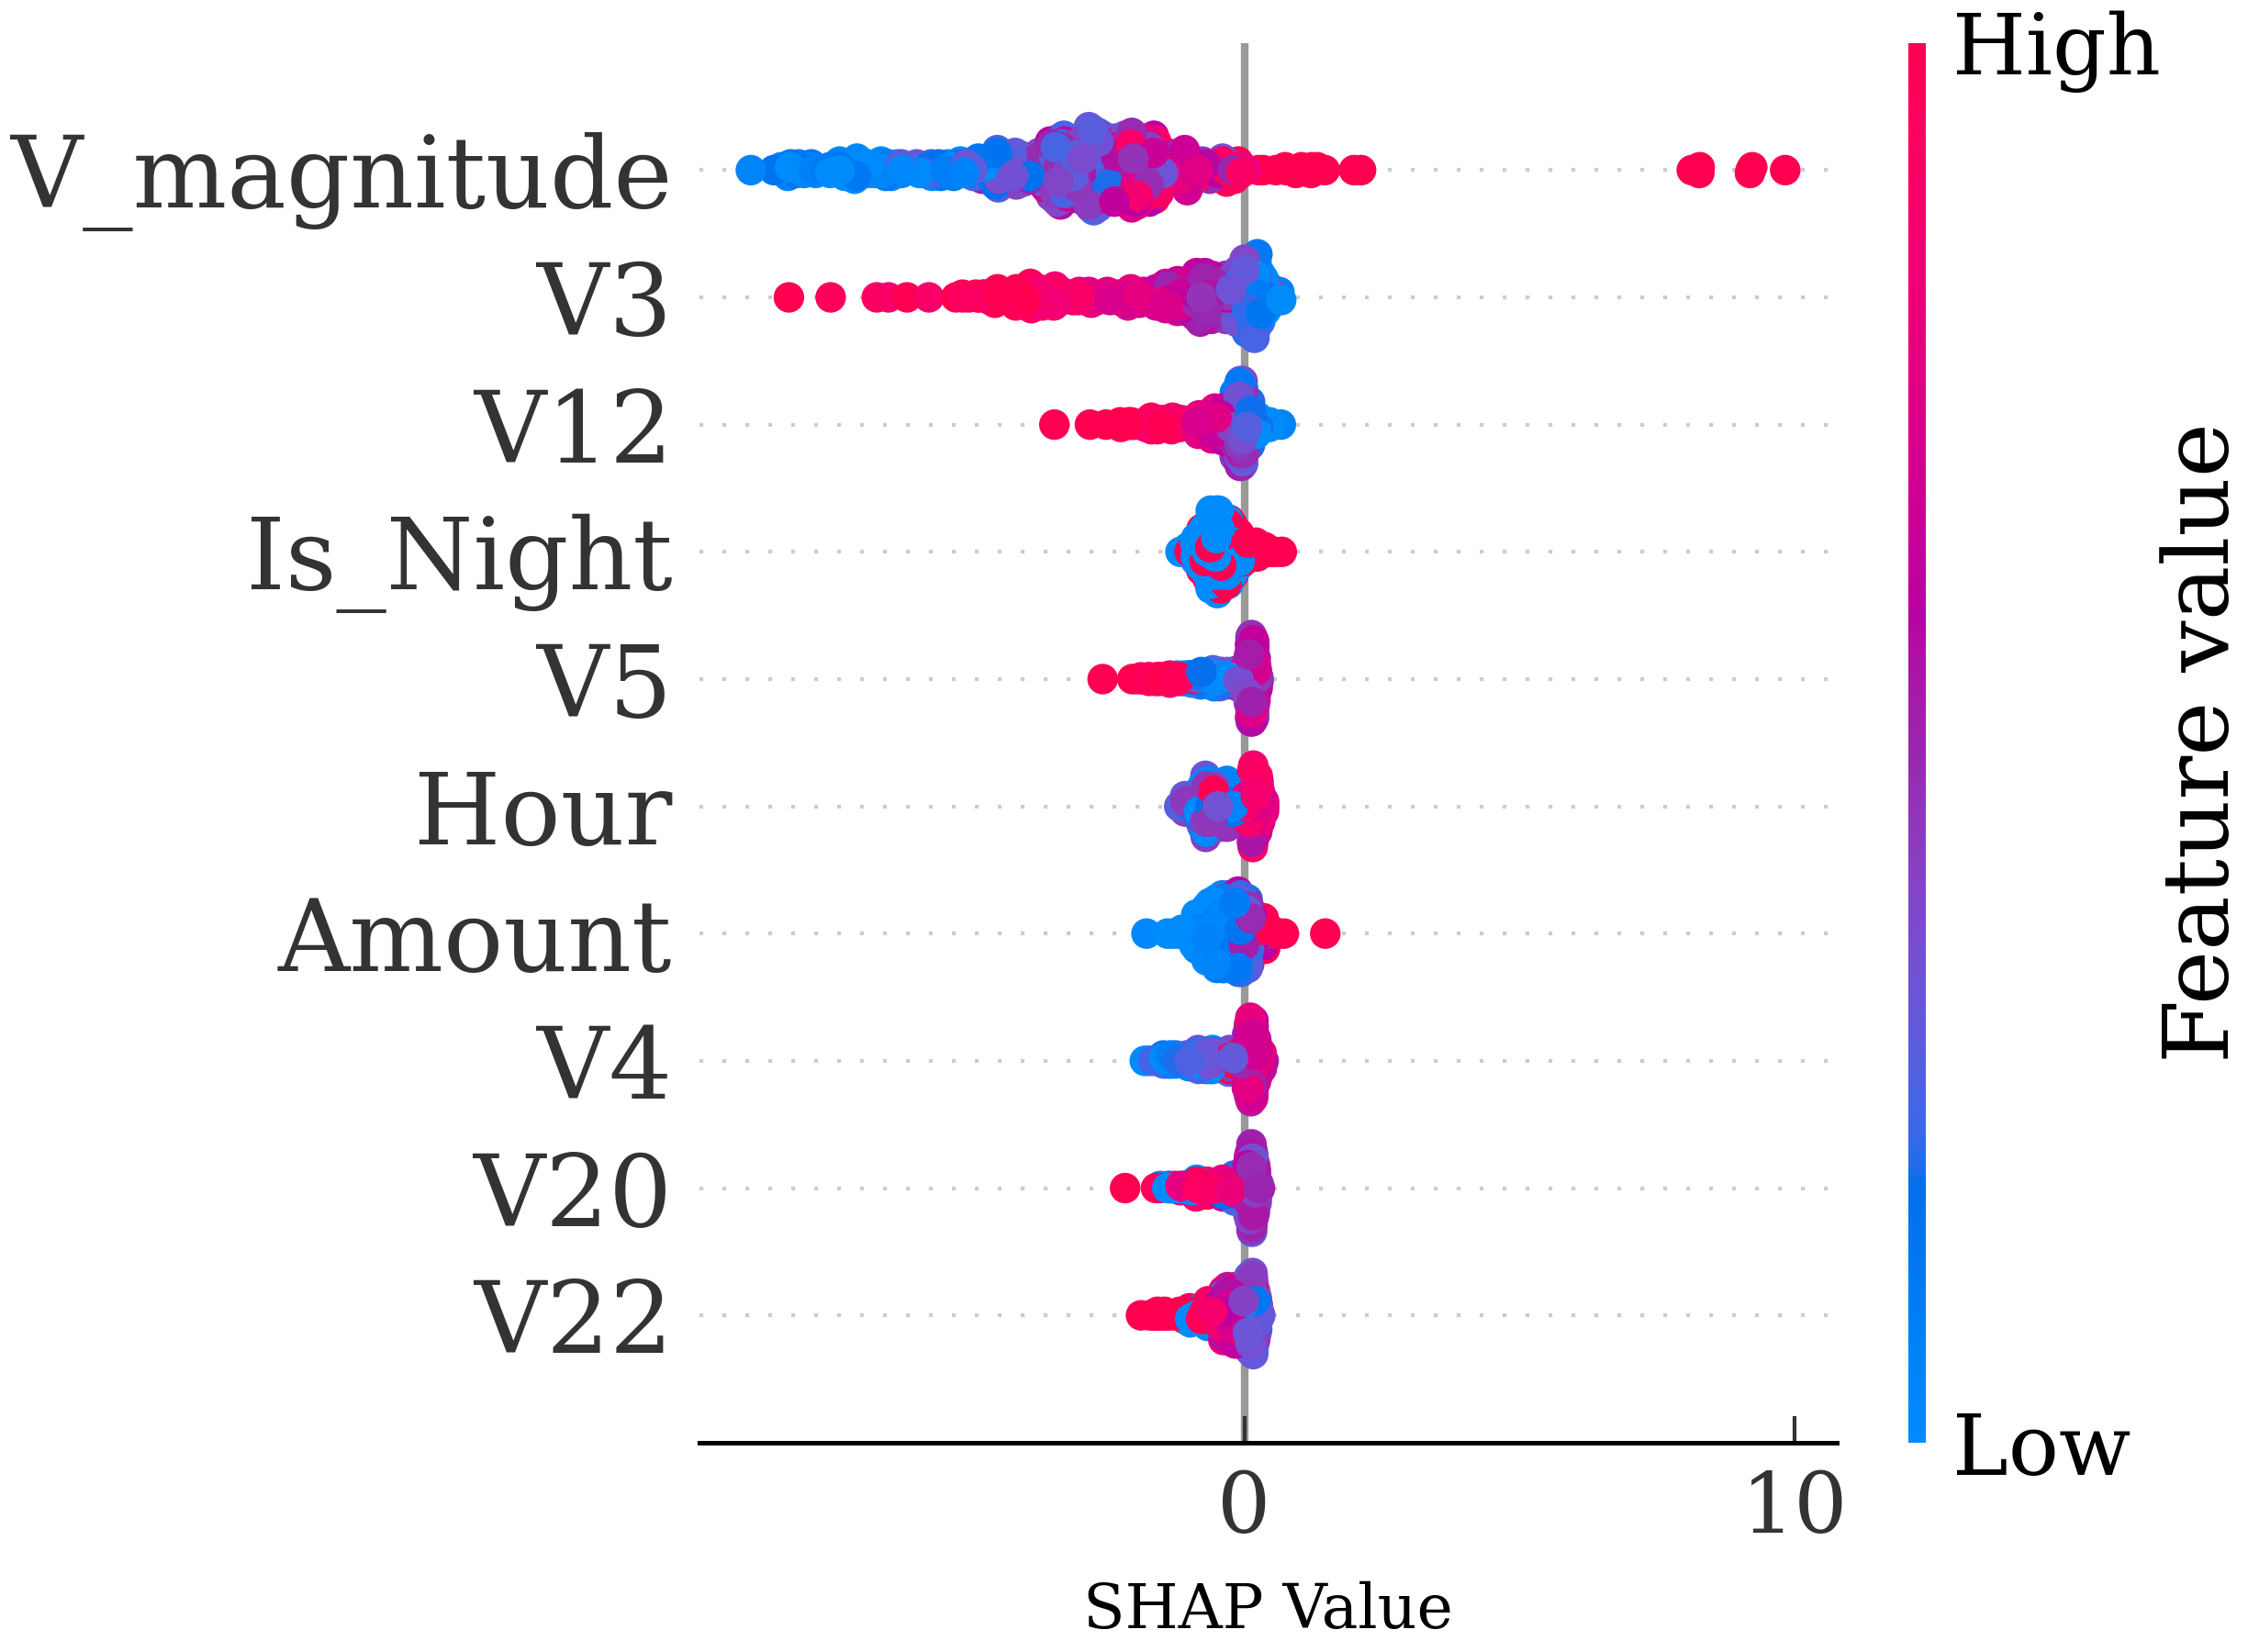
\includegraphics[width=\columnwidth]{fig08_shap_summary.png}
\caption{SHAP summary plot showing directional impact. Red indicates high feature values, blue indicates low values.}
\label{fig:shap_summary}
\end{figure}

\begin{table}[!t]
\centering
\caption{SHAP Explanations for Four Representative Transactions}
\label{tab:shap}
\begin{tabular}{@{}lcccc@{}}
\toprule
\textbf{Feature} & \textbf{TP\textsubscript{1}} & \textbf{TP\textsubscript{2}} & \textbf{FP} & \textbf{TN} \\
\midrule
Feature Energy   & +35\% & +28\% & +22\% & $-$12\% \\
PCA Comp. V3     & +22\% & +18\% & +8\%  & $-$8\% \\
Night Txn        & +18\% & +5\%  & +25\% & $-$3\% \\
Amount           & +15\% & +30\% & +12\% & $-$5\% \\
Other            & +10\% & +19\% & +33\% & +28\% \\
\midrule
\textbf{Score}   & \textbf{0.92} & \textbf{0.87} & \textbf{0.68} & \textbf{0.03} \\
\textbf{True Label} & Fraud & Fraud & Legit & Legit \\
\bottomrule
\end{tabular}
\end{table}

\subsection{Confusion Matrix Analysis}

Fig.~\ref{fig:cm} compares confusion matrices under static and dynamic thresholding. Dynamic thresholding reduces false negatives, directly translating to recovered fraud losses in production deployment.

\begin{figure}[!t]
\centering
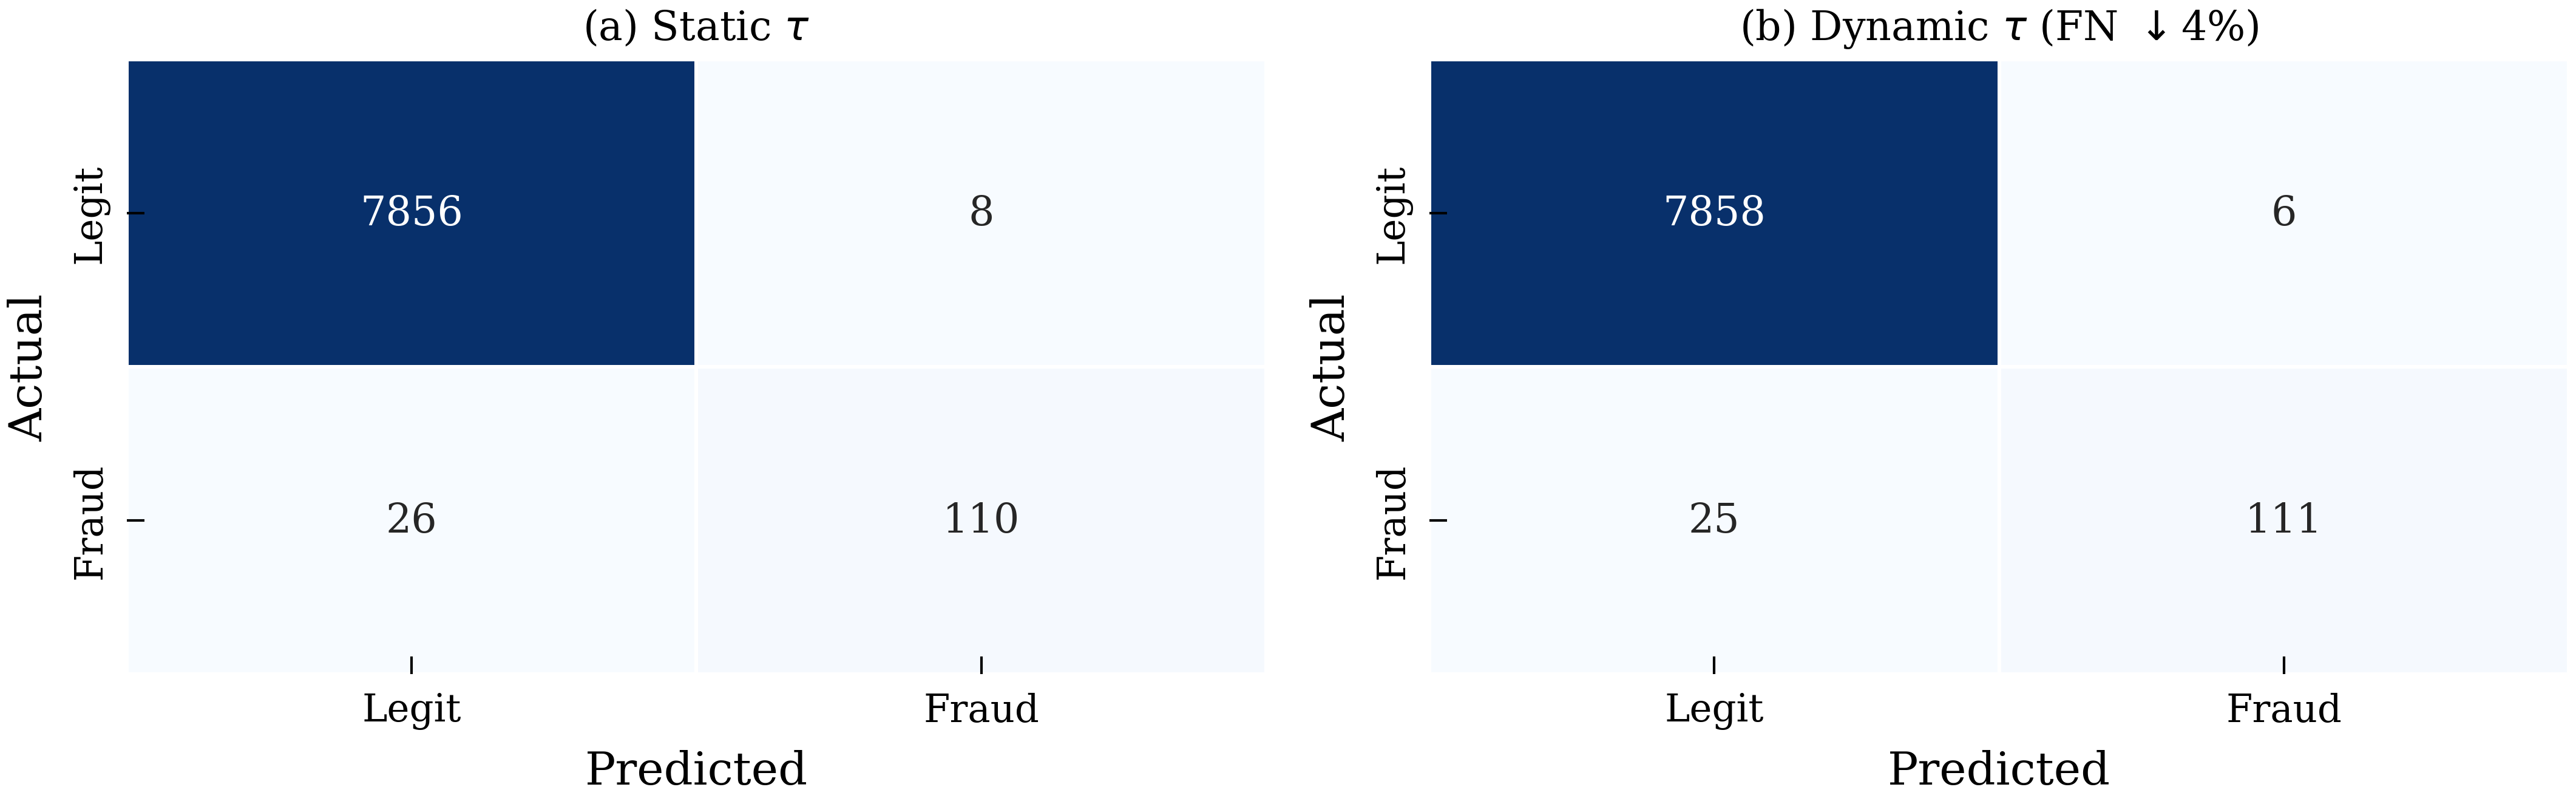
\includegraphics[width=\columnwidth]{fig06_confusion.png}
\caption{Confusion matrices under static (a) and dynamic (b) thresholding. Dynamic thresholding reduces false negatives while maintaining precision.}
\label{fig:cm}
\end{figure}

% ====================================================================
\section{Limitations and Future Work}
\label{sec:limitations}

The primary limitation of this study is the use of synthetic data. While the dataset replicates the statistical properties of the European Cardholder dataset~\cite{dal_pozzolo2015calibrating}, it may not fully capture the adversarial dynamics of real fraud evolution. Future work will validate on the European Cardholder dataset, the IEEE CIS Fraud Detection dataset, and the PaySim synthetic payments dataset to establish cross dataset generalizability.

The AADNN employs attention inspired feature interactions but does not implement a full Transformer encoder with multi head self attention, layer normalization, and positional encoding. Replacing the AADNN with a Tabular Transformer architecture would strengthen the theoretical contribution and may further improve performance on high dimensional transaction data.

The dynamic threshold currently requires labeled data in each temporal window for $F_1$ optimization. In production, labels arrive with delay (days to weeks). An unsupervised threshold adaptation mechanism based on distribution shift detection would make the approach more practical for real time deployment.

Additional promising directions include graph neural networks for modeling cardholder and merchant relationships, federated learning for privacy preserving multi bank deployment, and online learning for continuous model adaptation under concept drift.

% ====================================================================
\section{Conclusion}
\label{sec:conclusion}

This paper presented a hybrid AADNN Autoencoder framework for credit card fraud detection that addresses four critical limitations of existing systems: inability to detect novel fraud, static decision thresholds, cost agnostic optimization, and lack of explainability. The framework achieves the highest ROC AUC ($0.965 \pm 0.004$) among all evaluated methods and an $F_1$ of 0.886 under dynamic thresholding. The novel fraud simulation demonstrates that the Hybrid detects 46.9\% of unseen attack patterns where Random Forest achieves 0.0\% and XGBoost achieves 12.4\%, providing the strongest justification for the hybrid architecture. The ablation study confirms that fusion contributes +3.8\% AUC and dynamic thresholding adds +1.7\% $F_1$. SHAP analysis provides interpretable per transaction explanations identifying feature energy and temporal patterns as the dominant fraud indicators.

\bibliographystyle{IEEEtran}
\bibliography{references}

\end{document}
